\documentclass{article}
\usepackage{graphicx} % Required for inserting images
\usepackage{kotex}
\usepackage{amsmath}
\usepackage{mathtools}
\usepackage{amssymb}
\usepackage{amsthm}
\usepackage[margin=2cm,nonhead]{geometry}
\usepackage{setspace}   
\usepackage{abstract}
\usepackage{authblk}
\usepackage{enumitem}
\usepackage{float}
\usepackage{subcaption} % Recommended package for subfigures
\usepackage{multicol,layout,epsf,verbatim,array,tabularx,graphicx,kotex,amssymb,amsmath,setspace}
\usepackage{tikz}
\usetikzlibrary{
  hobby,
  intersections,
  spath3,
  decorations.markings,
  arrows.meta,
  }
\captionsetup[subfigure]{labelformat=empty}


\newcommand{\czero}{
  \tikz[baseline=-0.6ex, scale=0.7]{
    \path (0,0) coordinate (base);
    \draw[line width=0.7pt] (0,0.4) .. controls (0.3,0.3) and (0.3,-0.3) .. (0,-0.4);
    \draw[line width=0.7pt] (0.8,0.4) .. controls (0.5,0.3) and (0.5,-0.3) .. (0.8,-0.4);
  }
}
\newcommand{\cinf}{
  \tikz[baseline=1.2ex, scale=0.7]{
    \path (0,0) coordinate (base);
    \draw[line width=0.7pt] (0.4, 0) .. controls (0.2, 0.3) and (-0.2, 0.3) .. (-0.4, 0);
    \draw[line width=0.7pt] (0.4, 0.8) .. controls (0.2, 0.5) and (-0.2, 0.5) .. (-0.4, 0.8);
  }
}

\newcommand{\Xslashfront}{
  \tikz[baseline=-0.6ex, scale=0.28]{
    \draw[line width=0.7pt] (-1,1) -- (1,-1);
    \draw[line width=4.0pt, white] (-0.5,-0.5) -- (0.5, 0.5);
    \draw[line width=0.7pt] (-1,-1) -- (1,1);
  }
}

\newcommand{\Xslashback}{
  \tikz[baseline=-0.6ex, scale=0.28]{
    \draw[line width=0.7pt] (-1,-1) -- (1,1);
    \draw[line width=4.0pt, white] (-0.5,0.5) -- (0.5,-0.5);
    \draw[line width=0.7pt] (-1,1) -- (1,-1);
  }
}

\onehalfspacing

\newcommand{\rarrow}{\rightarrow}
\newcommand{\larrow}{\leftarrow}

\newtheorem{thm}{Theorem}
\theoremstyle{definition}
\newtheorem{defn}[thm]{Definition}
\theoremstyle{theorem}
\newtheorem{theorem}[thm]{Theorem}
\theoremstyle{proposition}
\newtheorem{prop}{Proposition}
\theoremstyle{corollary}
\newtheorem{corol}[thm]{Corollary}



\onehalfspacing
\setlength\parindent{0pt}


\renewcommand\Affilfont{\small}

\title{\textbf{Minimal Grid Diagrams of Theta-Curves and Handcuff Graphs up to 7 Crossings}}
\author[1]{Eunchan Cho}
\author[1]{Jeongwon Shin}
\author[1]{Boyeon Seo}
\author[1]{Minho Choi}
\author[2]{Hun Kim}
\author[3]{Gyotaek Jin}
\affil[1]{Researcher, Korea Scinece Academy of KAIST}
\affil[2]{Supervisor, Korea Science Academy of KAIST}
\affil[3]{Co-Supervisor, Department of Mathematical Sciences, Korea Advanced Institute of Scienceand Technology}


\renewcommand\Authands{ and }

\date{\vspace{-5ex}}

\begin{document}



\begin{center}
    {\LARGE \textbf{엇갈림수 7 이하의 세타커브와 수갑 그래프의 최소 그물 그림}\par}
    \vspace{0.3cm}
    {\large 조은찬\textsuperscript{1}, 신정원\textsuperscript{1}, 서보연\textsuperscript{1}, 최민호\textsuperscript{1}, 김훈\textsuperscript{2}, 진교택\textsuperscript{3}}\\
    {\large \textsuperscript{1}연구자, 한국과학영재학교 \par \textsuperscript{2}책임지도자, 한국과학영재학교 \par \textsuperscript{3}공동지도자, 한국과학기술원 수리과학과\par}

    \renewenvironment{abstract}
    {\begin{quote}
    \noindent \rule{\linewidth}{.5pt}\par{\bfseries \abstractname.}}
    {\medskip\noindent \rule{\linewidth}{.5pt}
    \end{quote}
    }

    \renewcommand{\abstractname}{초록}


    \begin{abstract}
        본 연구에서는 공간 그래프(spatial graph), 특히 엇갈림수(crossing number) $7$까지의 세타커브(theta-curve)과 수갑 그래프(handcuff graph)에서의 최소 그물 그림(minimal grid diagram)을 구함으로써 그들의 호 지수(arc index)를 확정시키고자 하였다. 또한 그 과정에서 호 지수의 상한과 하한을 구할 수 있었으며, 야마다 다항식(yamada polynomial)에 기반한 파이썬 프로그램을 작성하여 이를 확인해 보았다.\\ \\
        \textbf{중심어 : 세타커브, 수갑 그래프, 호 지수, 최소 그물 그림}
        \\
    \end{abstract}

    \vspace{1cm} % 한글/영문 사이 간격

    {\LARGE \textbf{Minimal Grid Diagrams of \\ Theta-Curves and Handcuff Graphs up to 7 Crossings}\par}
    \vspace{0.3cm}
    {\large Eunchan Cho\textsuperscript{1}, Jeongwon Shin\textsuperscript{1}, Boyeon Seo\textsuperscript{1}, Minho Choi\textsuperscript{1}, Hun Kim\textsuperscript{2}, Gyotaek Jin\textsuperscript{3}}\\
    {\large \textsuperscript{1}Researcher, Korea Science Academy of KAIST \par \textsuperscript{2}Supervisor, Korea Science Academy of KAIST\par \textsuperscript{3}Co-Supervisor, Department of Mathematical Sciences, Korea Advanced Institute of Science and Technology}
\end{center}

\renewenvironment{abstract}
{\begin{quote}
\noindent \rule{\linewidth}{.5pt}\par{\bfseries \abstractname.}}
{\medskip\noindent \rule{\linewidth}{.5pt}
\end{quote}
}

\begin{abstract}
Our purpose of this research is classifying theta-curves and handcuff graphs by their arc indices, which their crossing is up to 7.
We tried to find those arc indices by proving lower bounds and upper bounds of the theta-curves and handcuff graphs.
Also we programmed Python code that returns the minimal grid diagram of the theta curves and handcuff graphs which have crossing up to 7.
Yamada polynomial was used to prove bounds and programming the Python code.\\ \\
\textbf{Keywords : theta-curve, handcuff graph, arc index, minimal grid diagram}
\\
\end{abstract}

\newpage
\section{Introduction}
Knot theory is a field of mathematics that studies simple closed curves embedded in three-dimensional space. Study of theta-curves and handcuff graphs is included in knot theory. In this research, we tried to get the minimal grid diagrams of those graphs, which are up to 7 crossings.\\ \\
We first decided to use the Python code to examine the minimal grid diagrams of theta-curves and handcuff graphs. For this, we found the method to classify theta-curve and handcuff graphs by their Cromwell matrices, which are called THC matrices. Finding all possible matrices for those graphs and finding out the Yamada polynomial of each graphs could give the minimal grid diagram of the graph. \\ \\
Also, we used some mathematical methods to found out the minimal grid diagrams by using the bounds of the arc index, and used the Python code to examine if we found the right grid diagrams. Then we tried to decrease the gap of upper and lower bounds, and found out arc indices of some graphs.

\section{Theoretical Background}

\begin{defn}
    \textit{Theta-curve} is a spatial knot on $3$-sphere which has $2$ vertices and $3$ edges. 
\end{defn}
\begin{defn}
    \textit{Handcuff graph} consists of $2$ loops and $1$ edge joining the loops.
\end{defn}

\begin{figure*}[h]
    \centerline{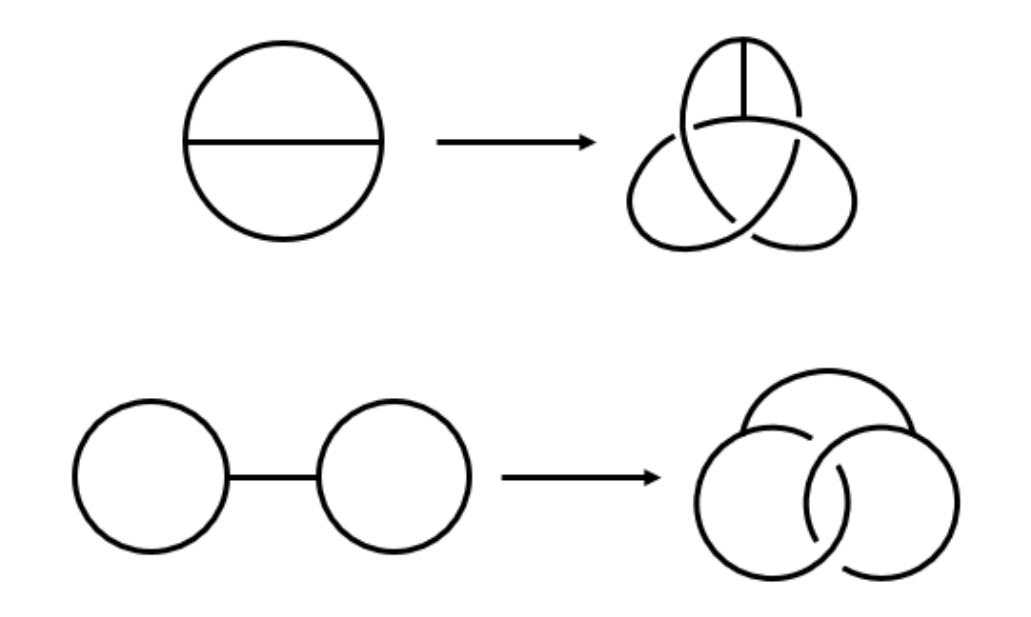
\includegraphics[width=0.3\textwidth]{figure/theta and handcuff graph.png}}
    \caption{Examples of theta-curves and handcuff graphs.}
    \label{figure_1} 
\end{figure*}

In the projection of the handcuff graph and theta-curve, the section where they meet themselves is named \textit{crossing}. 
For each handcuff graphs and theta-curves, the minimal number of crossings are called the \textit{crossing number}.
If the one graph and other graph's continuous transform of the graph is same, these graphs are \textit{equivalent}. 
The \textit{Generalized Reidemeister Moves} are used to transfrom a projection of handcuff graphs and theta-curves.\\

\begin{figure*}[h]
    \centerline{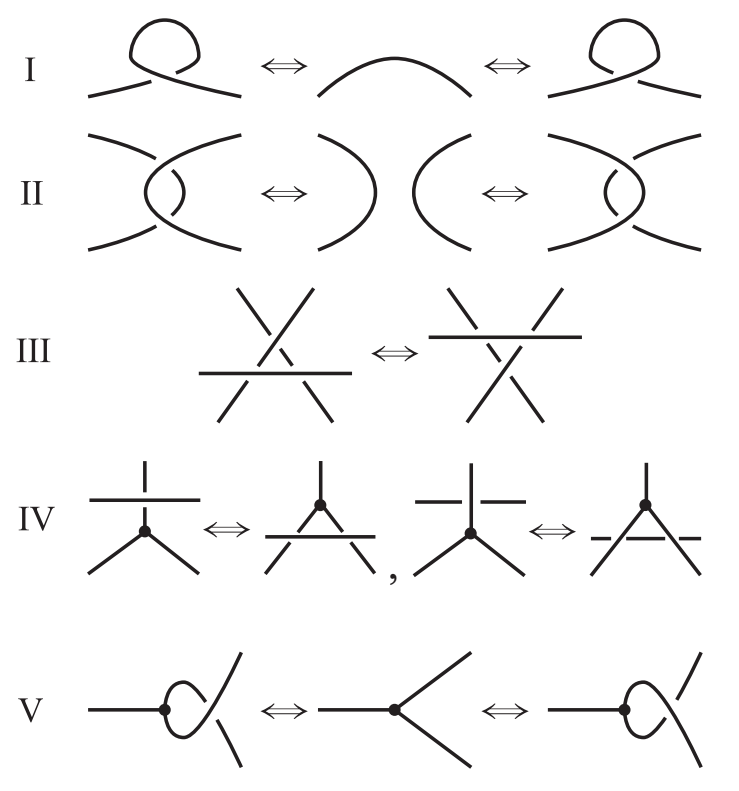
\includegraphics[width=0.5\textwidth]{figure/reidemeister.png}}
    \caption{Generalized Reidemeister moves.}
    \label{figure_1} 
\end{figure*}

A theta-curve is said to be trivial if it can be embedded in a $2$-sphere in $S^3$.
In the similiar way, a handcuff graph is said to be trivial if it can be embedded in a $2$-sphere in $S^3$.

\begin{figure*}[h]
    \centering
    \subfloat{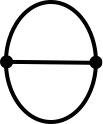
\includegraphics[width=0.1\textwidth]{figure/y6.png}}
    \hspace{0.05\linewidth}
    \subfloat{
\includegraphics[width=0.25\textwidth]{figure/y7.png}}
    \caption{Trivial theta-curve and handcuff graph.}
    \label{figure_1} 
\end{figure*}

\begin{defn}
    \textit{Arc presentation} is an open-book decomposition of $\mathbb{R}^3$ which has open half-planes as pages and the standard z-axis as the binding axis.
\end{defn}

Every spatial graph $G$ can be embedded in an open-book decomposition with finitely many pages so that it meets each page in exactly one simple arc with two different end-points on the binding axis.
In knot theory, \textit{arc index}, is the minimal number of pages among all possible arc presentations of graph. This arc presentation with the minimal number of pages is \textit{minimal arc presentation.} \textit{Prime knots} are knots that is not constructed by combining simpler knots. We are finding the arc index for the prime theta-curve and handcuff graph up to seven crossings.

\begin{figure*}[h]
    \centering
    \subfloat{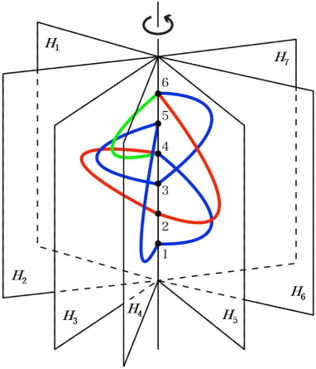
\includegraphics[width=0.33\textwidth]{figure/openbook.png}}
    \subfloat{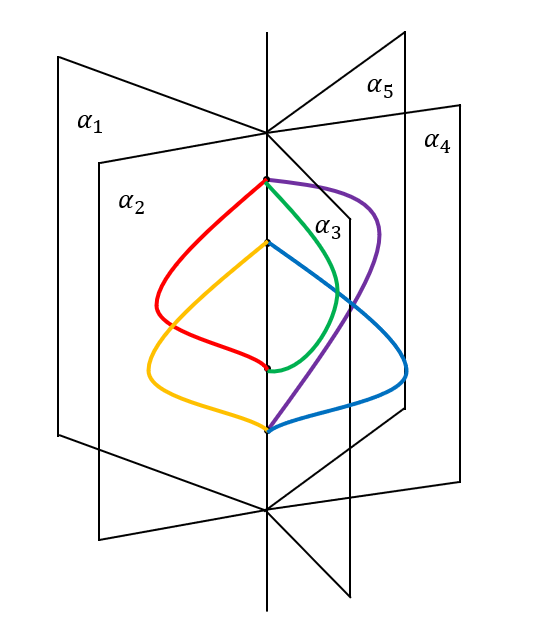
\includegraphics[width=0.37\textwidth]{figure/handcuff_openbook.png}}
    \caption{Arc presentation of theta-curve $3_1$ and a trivial handcuff graph}
    \label{figure_1} 
\end{figure*}


\begin{defn}
    The \textit{grid diagram} is a handcuff graph or theta‐curve diagram of vertical strands and one less number of horizontal strands with the properties that at every crossing the vertical strand crosses over the horizontal strand and no two horizontal segments are co‐linear and no two vertical segments are co‐linear.
\end{defn}

\begin{defn}
   The \textit{Cromwell matrix} is an $n \times n$ binary matrix each of whose rows and columns has exactly two 1s. 
   For theta‐curve and handcuff graph, its Cromwell matrix is called the 
   the \textit{THC-Cromwell matrix} is the matrix that satisfies the following conditions.
\end{defn}
\begin{enumerate}
    \item It is a binary $n\times(n+1)$ matrix.
    \item It has exactly two 1s in every column.
    \item There are only three 1s in two distinct rows (which are called the \textit{Three-row}) and every other rows has exactly two 1s.
\end{enumerate}

If the 1s of the Cromwell matrix are connected by horizontal and vertical lines with vertical lines are always on the horizontal lines, it leads to the grid diagram. The arc presentation can be expressed by grid diagram and vice versa. They are in one-to-one correspondence. Also, if the number of half planes in arc presentation is $\alpha$, then the size of corresponding grid diagram is $(\alpha - 1) \times \alpha$.\\

\begin{figure*}[h]
    \centerline{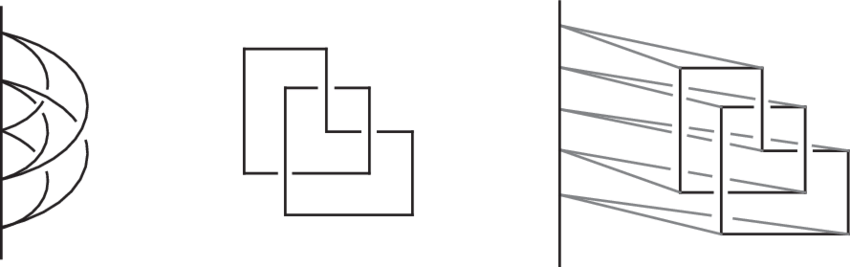
\includegraphics[width=0.5\linewidth]{An arc presentation and a grid diagram of the knot.png}}
    \caption{An arc presentation and a grid diagram of the knot}
    \label{figure_2}
\end{figure*}

\begin{theorem}
    Arc presentations exist for every theta-curve and handcuff graph. 
\end{theorem}
\begin{proof}
    For any theta-curve and handcuff graph, we can put it on a grid by using some suitable planar isotropy.
    Then for every crossing it has, there are only two following cases. \\
    \begin{figure*}[h]
        \centerline{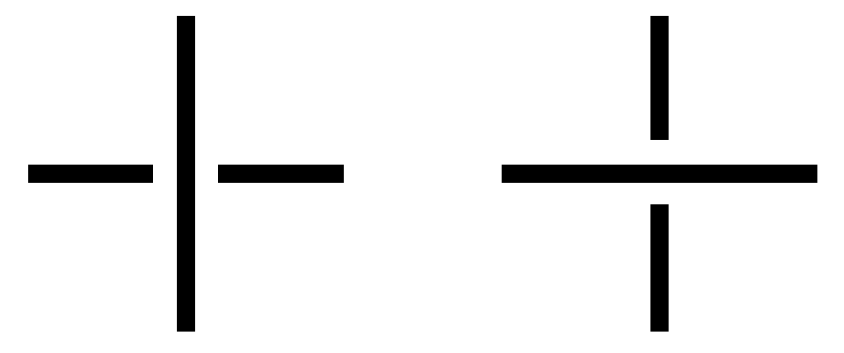
\includegraphics[width=0.5\linewidth]{figure/crossings.png}}
        \caption{Cases for crossings}
        \label{figure_2}
    \end{figure*}
    \\ For each crossings, if it is a first case, then it is over.
    However, if it is a second case, then we can make that crossing to first case using some suitable movement. \\
    \begin{figure*}[h]
        \centerline{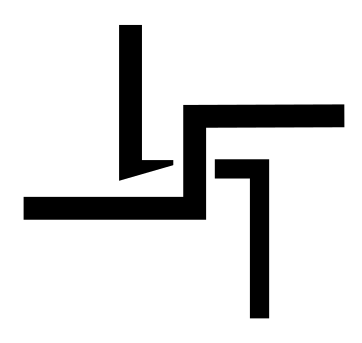
\includegraphics[width=0.25\linewidth]{figure/move crossing.png}}
        \caption{Suitable movement for case 2}
        \label{figure_2}
    \end{figure*}
    \\ Therefore, it becomes the grid diagram and since the grid diagrams and arc presentations are in one-to-one correspondence, there always exists arc presentations for every theta-curve and handcuff graph.
\end{proof}

\begin{defn}
    The \textit{link with $n$-components} is an embedding of the disjoint union of $n$ circles $S^1 \cup \cdots \cup S^1$ in $\mathbb{R}^3$. $1$-component link is called a \textit{knot}.
\end{defn}

The polynomial of the knot is invariant. \textit{Yamada polynomial} is invariant when it is mulitplied $(-x)^n$ for some integer n. The \textit{spread} of a knot, is substraction of maximal degree of minimal degree of the polynomial. It is a invariant since Yamada polynomial is invariant when mulitplied by $(-x)^n$.\\

Let 3 edges of theta-curve is $e_1, e_2, e_3$, then $e_1 \cup e_2$, $e_2 \cup e_3$, $e_3 \cup e_1$ becomes a knot on 3-sphere. This knots are \textit{consituent knot} of the theta-curve.

\begin{defn}
    \textit{Stacked tangle} of an theta-curve and handcuff graph is stacked disks each with the frame as boundary with following properties:
\end{defn}
\begin{itemize}
\item Only two disk called \textit{non-simple disks} contain one vertex and three line
segments which joins the vertex and boundary point.
\item One of the non-simple disks is at the top.
\item Other disks called \textit{simple disks} contain simple arc which joins two
points on the boundary.
\item When view from above
\begin{itemize}
    \item two arcs in different simple disks intersect at most one point (by RII)
    \item arc in simple disk and tree in non-simple disk intersect at most one
point (by RV)
\end{itemize}
\end{itemize}

\textit{Simple closure} of stacked tangle is a stacked tangle with \textit{caps} satisfying following properties:
\begin{itemize}
    \item A \textit{cap} is a simple arc in outside of stacked tangle joining end points of arcs or line segments
    \item When view from above any tow caps have no intersection.
\end{itemize}
Then a simple closure of a stacked tangle without any nested caps is
corresponding to an arc presentation.\\

A \textit{reduced simple closure of a stacked tangle} is
\begin{itemize}
    \item a simple closure of a stacked tangle without any nested caps
    \item any two arcs(including line segment) joining by caps have no intersection when view from above
\end{itemize}

%\begin{proof}
%$$\alpha(\theta) \leq c(\theta) + e + b$$ when e is number of edges, b is number of bouquet cut-components. We have 3 edges, 0 bouquet cut-componentes for theta-curves. Therefore, $$\alpha(\theta) \leq c(\theta) + 3.$$
%\end{proof}

\section{Research Methods and Procedure}
First, we made a Python Code to find the arc index and the cromwell matrix of the knots. Then we used the upper and lower bounds, and also found the smaller upper bounds and larger lower bounds. Finally we used the direct method to find the arc index by drawing the binding circle.

\subsection{The Python Code}
The Python code generates the possible Cromwell matrices of theta-curves and handcuff graphs, and compares with the existing ones in the table which is less or equal to 7 crossings.
It eventually returns the Cromwell matrix of the compared theta-curve and handcuff graph.
To distinguish the Cromwell matrices from theta-curves and handcuff graphs, which is generated and removed by the rules from the above section, we should use the determinant of the Cromwell matrices.\\
%\begin{defn}
%The \textit{grid diagram} of a knot is a projection that consists only of horizontal and vertical lines, and the vertical line always passes above the horizontal line. (However, in this case, there must be exactly two points (excluding the vertices) that are vertically bent for each horizontal line (row) and vertical line (column), and the two vertices must be on the horizontal line.)
%\end{defn}

%\begin{theorem}
%Every theta-curve and handcuff graph has its corresponding THC-Cromwell matrix.
%\end{theorem}
\begin{defn}
    Let any THC-cromwell matrix G. Consider any Three-row $i$ and its three 1s, $a_{ij}, a_{ik}, a_{il}$, which means that $a_{ij} = a_{ik} = a_{il} = 1$. The \textit{H-deletion Matrix} of the THC-cromwell matrix G is $(n-1)\times(n-1)$ matrix which deleted row $i$ and column $j$, $k$ (which are called the \textit{edge-columns}) from the matrix G\\
\end{defn}

\begin{figure*}[h]
    \centerline{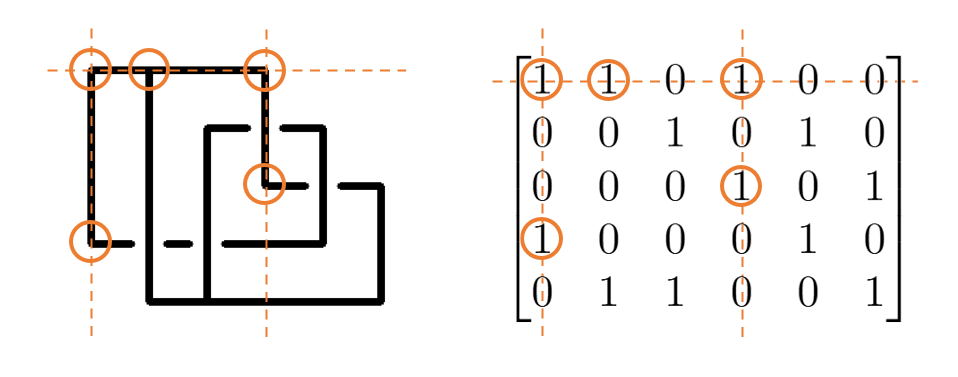
\includegraphics[width=0.5\textwidth]{figure/Hdeletion.png}}
    \caption{H deletion of THC-matrix of theta-curve $3_1$.}
    \label{figure_1} 
\end{figure*}

\subsubsection{Main Theorem}
\begin{theorem}The given THC-Cromwell matrix is theta-curve if and only if determinant of the H-deletion matrix is $\pm 1$.The given THC-Cromwell matrix is handcuff graph if and only if determinant of the H-deletion matrix is 0 or $\pm 2$.
\end{theorem}

\begin{proof}
\begin{enumerate}
    \item \textbf{Determinant of the cromwell matrices of Knot}\\
    The cromwell matrix of a knot is a $n\times n$ binary matrix which has exactly two 1s for each rows and columns
    We are interested of the determinant of the cromwell matrix of knots, so we are going to use the row and column operations to get simpler matrix.
    In this way, determinant of the Cromwell matrix would change only by multiplying $\pm 1$.\\
    Now we follow these steps : \\
    \begin{enumerate}
        \item Since there are always exactly two 1s in every row, there exists two columns that containing the 1s of the top row. Using column operations, interchange those two columns with the left most and secondary left most columns of the matrix.
        \item Choose secondary column from the left. It should contain another 1 below the 1 which is from the top row, so interchange a row containing that below 1 with secondary top row by using row operations.
        \item Cover the left most column and top row and repeat (a), (b) (What you need to careful is that when you interchange the row, you should also change the covered elements together.) until we get the following matrix.
    \end{enumerate}
    
    $$\begin{pmatrix} 
    1 & 1 & 0 & \cdots & 0\\
    0 & 1 & 1 &  &  \\
    0 & 0 & 1 & & \vdots\\ 
    \vdots & & & \ddots & \\
    1 & 0 & \cdots & 0 & 1
    \end{pmatrix}$$
Next, we apply the row operation. We add each row above the bottom row to the bottom row.
    $$\begin{pmatrix} 
    1 & 1 & 0 & \cdots & 0\\
    0 & 1 & 1 &  &  \\
    0 & 0 & 1 & & \vdots\\ 
    \vdots & & & \ddots & \\
    2 & 2 & \cdots & 2 & 2
    \end{pmatrix}$$
If n is even, by subtracting bottom row with &2R_1, 2R_3, ... , 2R_{n-1}$ We can get a matrix like
    $$\begin{pmatrix} 
    1 & 1 & 0 & \cdots & 0\\
    0 & 1 & 1 &  &  \\
    0 & 0 & 1 & & \vdots\\ 
    \vdots & & & \ddots & \\
    0 & 0 & \cdots & 0 & 0
    \end{pmatrix}$$
Since the last row is zero row, the determinant is 0. \\
If n is odd, by subtracting bottom row with $2R_1, 2R_3, ... 2R_{n-2}$, we can get a following matrix. 
    $$\begin{pmatrix} 
    1 & 1 & 0 & \cdots & 0\\
    0 & 1 & 1 &  &  \\
    0 & 0 & 1 & & \vdots\\ 
    \vdots & & & \ddots & \\
    0 & 0 & \cdots & 0 & 2
    \end{pmatrix}$$
Since it is upper triangular matrix, we can obtain determinant by trace. Hence the other entry is all 1, the determinant is $\pm 2$.\\

\item \textbf{Proof in the case of theta-curve}\\
Since the THC-cromwell matrix is not a $n\times n$ matrix, we consider H-deletion matrix of THC-cromwell matrix. 
Now, we are going to count n, which is the number of times $1$s in edge-columns is included in Three-rows.
\begin{enumerate}
    \item \textbf{When $n = 0$}\\
    T-shaped figure is given.
    \item \textbf{1 (middle vertex)}\\
    Line-shaped figure is given.
    \item \textbf{1 (end vertex)}\\
    Line-shaped figure is given.
    \item \textbf{2 (two end vertices)}\\
    T-shaped figure is given.
    \item \textbf{2 (middle and end vertices)}\\
    Line-shaped figure is given.
\end{enumerate}

\begin{enumerate}[label={(\roman*)}]
    \item \textbf{Line-shaped figure}\\
    Let the matrix is given.
    $$\begin{pmatrix}
        1 & 1 & 1 & 0\\
        0 & 1 & 1 & 1\\
        1 & 0 & 0 & 1
    \end{pmatrix}$$
    If you work on deleting rows and columns here, you can get the line-shaped figure of the following figure. If you convert this into a matrix according to the previous section,
    $$\begin{pmatrix}
        1 & 1 \\
        0 & 1
    \end{pmatrix}$$
    is given.\\
    If we appropriately perform adding multiple of one row to another row and replacing the second row with the result, the determinant changes only by $\pm 1$, and the resulting matrix will be identity matrix. If we appropriately transform other theta-curves, we can get the same result.
    \item \textbf{T-shaped figure}\\
    Let the matrix is given.
    $$\begin{pmatrix}
        1 & 1 & 1\\
        1 & 1 & 1\\
    \end{pmatrix}$$
    If you work on deleting rows and columns here, you can get the T-shaped figure of the following figure. If you convert this into a matrix according to the previous section,
    $$\begin{pmatrix}
        1 & 1 & 1\\
        0 & 1 & 0\\
        0 & 0 & 1
    \end{pmatrix}$$
    is given.\\
    If we appropriately perform adding multiple of one row to another row and replacing the second row with the result, the determinant changes only by $\pm 1$, and the resulting matrix will be identity matrix. If we appropriately transform other theta-curves, we can get the same result.
\end{enumerate}
Therefore, $\pm 1$ will be the determinant of the theta-curve's H-deletion matrix.

\item \textbf{Proof in the case of handcuff graph}\\
    Do the H-deletion. Then, we can make the matrix of this grid diagram by upper section. If end vertices is erased when we delete the row, then by what vertices is erased in the other three vertices row in the grid diagram can make different matrix.
    \begin{enumerate}
        \item \textbf{0}\\
        Knot is given.
        \item \textbf{1 (middle vertex)}\\
        Line-shaped figure is given.
        \item \textbf{1 (end vertex)}\\
        It is not given since one column might have 3 vertices.
        \item \textbf{2 (two end vertices)}\\
        It is not given since rows which have 3 vertices is connected with 2 line.
        \item \textbf{2 (middle and end vertices)}\\
        It is not given since rows which have 3 vertices is connected with 2 line.
    \end{enumerate}
    
    \begin{enumerate}[label={(\roman*)}]
        \item \textbf{Knot}\\
        By upper section, the determinant becomes 0 or $\pm 2$.
        \item \textbf{Line-shaped figure}
        Let the matrix is given.
        $$\begin{pmatrix}
            0 & 0 & 0 & 1 & 1\\
            0 & 1 & 0 & 1 & 1\\
            1 & 1 & 1 & 0 & 0\\
            1 & 0 & 1 & 0 & 0
        \end{pmatrix}$$
        If you work on deleting rows and columns here, you can get the line-shaped figure of the following figure. If you convert this into a matrix according to the previous section,
        $$\begin{pmatrix}
            1 & 1 & 0 \\
            0 & 1 & 1 \\
            0 & 0 & 0 \\
        \end{pmatrix}$$
        Since it is upper triangular matrix, the determinant of the matrix is trace, so the determinant of this matrix is 0.
    \end{enumerate}
\end{enumerate}
\end{proof}

\subsection{Bounds of Arc Index}
We found the bounds of arc index by the theoretical background, or we found the new bounds inspired by the theoretical background.


\begin{theorem}
Let T be any theta-curve and $K_1$, $K_2$, $K_3$ be three constituent knots of T. Then $$\alpha(T) \geq \underset{i \in \{1,2,3\}}\max \alpha(K_i) + 1.$$
\end{theorem}

\begin{theorem}
Let T be any theta-curve and $K_1$, $K_2$, $K_3$ be three constituent knots of T. Then $$\alpha(T) \geq \frac{1}{2}\sum_{i=1}^3\alpha(K_i).$$
\end{theorem}

\begin{theorem}
For any theta-curve $\theta$, $$\alpha(\theta)\geq\frac{1+\sqrt{f(\alpha(\theta))+36c(\theta)}}{3} \left(f(x) = \begin{cases} 
		73 & x \equiv 0 \pmod 6\\ 
		4 & x \equiv 1 \pmod 6\\ 
		25 & x \equiv 2 \pmod 6\\ 
		-8 & x \equiv 3 \pmod 6\\ 
		49 & x \equiv 4 \pmod 6\\ 
		20 & x \equiv 5 \pmod 6\\ 
     \end{cases} \right).$$
\end{theorem}

\begin{theorem}
For theta-curve $\theta$, if $c(\theta)$ is the crossing number, then $$\alpha(\theta) \leq c(\theta) + 3.$$
\end{theorem}

\begin{theorem}
Let T be any theta-curve. Then $$2+\sqrt{\max\deg_x R(S_T) - \min\deg_x R(S_T) + 4} \leq \alpha(T)$$ where $R(T)$ is a Yamada polynomial of the theta-curve T, and $S_{T}$ be a reduce simple closure of stacked tangle of a theta-curve T corresponding to minimal arc presentation of T.
\end{theorem}
\begin{defn}
    The \textit{non-simple cap} is the cap that connects simple disk and non-simple disk or two non-simple disks.
\end{defn}

\begin{theorem}
The number of the simple cap of the graph $G$ is invariant if least one of the edges are not crossed with others when the projection has minimal crossing, except the trivial theta-curve.
\end{theorem}
\begin{proof}
     To find the number of the non-simple cap from the grid diagram, we can draw the horizontal lines which include 1 from row that has three 1s. Since non-simple cap connects 1s from rows which have three 1s, the number of horizontal lines is the number of the non-simple caps. When the edge that directly connects two vertices is not crossed, the number of edges that starts from the vertices, which is 5, is the number of the horizontal lines. It can be shown by drawing the binding circle of the knot. Since the binding circle crosses the crossed area of two other edges, the number of edges that starts from the vertices is 5, 2 from each vertices and 1 that directly connects the vertices, except the trivial theta-curve. Since $\alpha(G))$ is the number of caps, the number of simple cap is $\alpha(G) - 5$.\\
\end{proof}

\begin{defn}
    In a handcuff curve, the \textit{vertex edge} is an edge that is connected to both vertices.
\end{defn}

\begin{defn}
    In a handcuff curve, the \textit{link component} is a union of the loops from each vertex to itself.
\end{defn}

\begin{theorem}[Cromwell, P. R.]
    If $L$ is an alternating and non-split link, then
    \[ \alpha(L) = c(L)+2. \]
    %crossing number 정의를 써야하나???
\end{theorem}

\begin{theorem}[Lee, M. J., No, S., \& Oh, S.]
    For any spatial graph $H$,
    \[ \alpha(H) \leq c(H)+e+b, \]
    where $e$ is the number of the edge and $b$ is the number of the bouquet.
\end{theorem}

\begin{corol}
    If $H$ is a handcuff curve,
    \[ \alpha(H) \leq c(H)+5. \]
    Especially, if the link component of $H$ is non-split,
    \[ \alpha(H) \leq c(H)+3. \]
\end{corol}

\begin{proof}
    If $H$ is a handcuff curve, the number of the edge is $3$, and the number of the bouquet is at most $2$. Thus the first inequality holds since $e=3, b \leq 2$. If there is a bouquet, one of the loops can be pulled out without affecting the rest. (See figure 1.) Then, if we remove the vertex edge of $H$, the remaining link component is a split link. Thus there are no bouquet if the link component of $H$ is non-split, and we have second inequality since $e=3, b=0$.
\end{proof}

\begin{figure*}
    \centerline{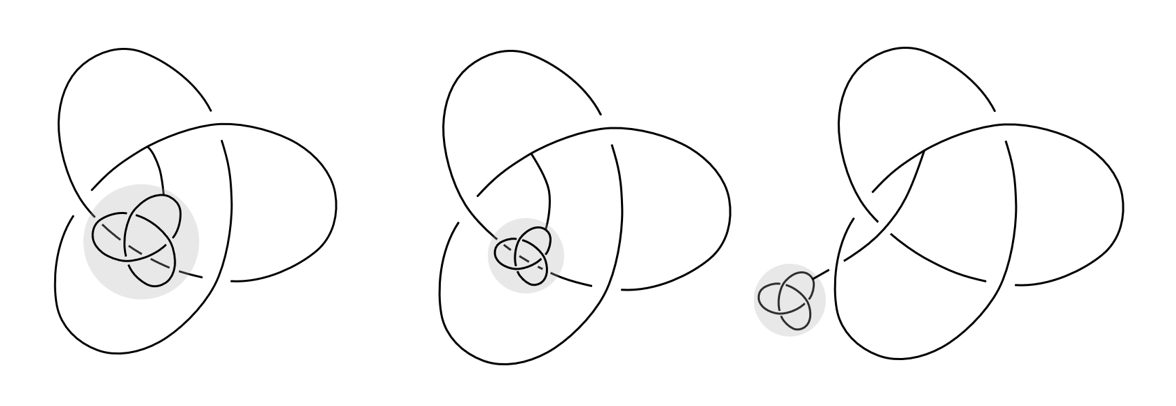
\includegraphics[width=\textwidth]{image.png}}
    \caption{caption}
    \label{figure_4} 
\end{figure*}

\begin{prop}
    For a handcuff curve $H$, let $L$ be a link component of $H$. Then,
    \[ \alpha(H) \geq \alpha(L)+1. \]
\end{prop}
\begin{proof}
    In the arc presentation of $H$, let $v_1$, $v_2$ be the vertices of $H$. Then, there are half-planes that contain the vertex edge of $H$. If we remove them, the remainder is the arc presentation of $L$, the link component of $H$. Since the number of half-planes that contain the vertex edge is at least $1$, we obtain
    \[ \alpha(H) \geq \alpha(L) + (\text{the number of half plane that contain vertex edge}) \geq \alpha(L)+1. \]
\end{proof}

Using the Theorem 1, we obtain the following corollary.

\begin{corol}
    In the handcuff curve, if the link component $L$ is alternating and non-split, then
    \[ \alpha(H) \geq c(L)+3. \]
\end{corol}

\begin{proof}
    Since $L$ is alternating and non-split link, $\alpha(L)=c(L)+2$ by Theorem 1. Thus, \[\alpha(H) \geq \alpha(L)+1 = \left( c(L)+2 \right)+1 = c(L)+3\] according to Proposition 1.
\end{proof}

Combining the above corollary and the corollary of Theorem 2, we have the following theorem.

\begin{theorem}
    For the handcuff curve $H$, if the link component $L$ is alternating and non-split, then
    \[ \alpha(H) = c(L)+3. \]
\end{theorem}

We now consider the Yamada polynomial of the handcuff curve and investigate the relationship between the difference of its maximum and minimum degrees and the arc index.

\begin{defn}
    For a graph $G=(V, E)$, where $V$ is vertex set of $G$ and $E$ is edge set of $G$, let us define $2$-variable Laurent polynomial
    \[ h(G)(x, y) = \sum_{F \subset E} (-x)^{-|F|} x^{\mu(G-F)} y^{\beta(G-F)} \]
    where $\mu(G)$ and $\beta(G)$ is the number of connected components of $G$ and the first Betti number of $G$. \\
    Then, the Yamada polynomial of a graph $G$, $R(G)$ is defined by
    \[ R(G)(x) = h(G)(-1, -x-2-x^{-1}). \]
\end{defn}

It is known that, for some integer $n$, the product $(-x)^n R(G)$ (where $R(G)$ is the Yamada polynomial of the spatial graph $G$) is an ambient isotopy invariant. Moreover, the Yamada polynomial satisfies the following properties.

\begin{theorem}
    For the Yamada polynomial, the following properties hold.
    \begin{enumerate}
        \item $R( \cdot ) = -1$
        \item Let $e$ be a non-loop edge of a graph $G$. Then, $R(G) = R(G / e) + R(G - e)$, where $G/e$, $G-e$ denote the graphs obtained by contracting and deleting the edge $e$, respectively.
        \item Let $e$ be a loop edge of a graph $G$. Then, $R(G) = -(x+1+x^{-1}) R(G-e)$.
        \item Let $G_1 \cup G_2$ be a disjoint union of graphs $G_1$ and $G_2$. Then, $R(G_1 \cup G_2) = R(G_1)R(G_2)$.
        \item Let $G_1 \cdot G_2$ be a union of graphs $G_1$ and $G_2$ having one common point. Then, $R(G_1 \cdot G_2) = -R(G_1)R(G_2)$.
        \item If $G$ has an isthmus, then $R(G)=0$.
    \end{enumerate}
\end{theorem}

\begin{theorem}
    For the Yamada polynomial, the following properties hold.
    \begin{figure*}[h]
        \centerline{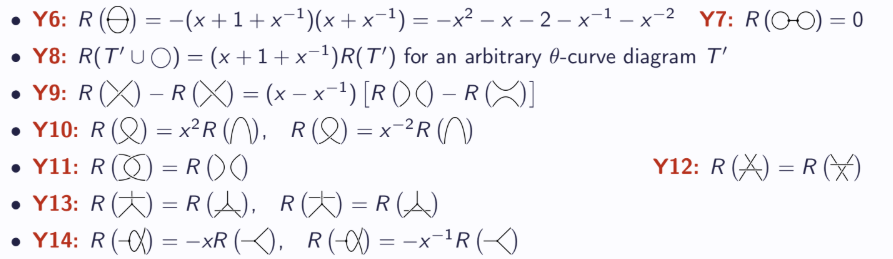
\includegraphics[width=0.75\linewidth]{yamada_property.png}}
        \caption{Properties of Yamada polynomial.}
        \label{figure_3}
    \end{figure*}
\end{theorem}

Now, using the stacked tangle representation and the Yamada polynomial, we will prove the following theorem. The following theorem gives a lower bound for the arc index in terms of the Yamada polynomial.

\begin{theorem}
    Let $S_T$ be the closure of stacked tangle of theta curve or handcuff curve. Then,
    \[ \text{spr}(R(S_T)) \leq 2n+2 \]
    where $n$ is the number of crossings in $S_T$ and $\mathrm{spr}(f)$ denotes the spread of $f$.
\end{theorem}

\begin{corol}
    If $G$ is a theta curve or handcuff curve, then
    \[ \alpha(G) \geq \frac{5 + \sqrt{4 \mathrm{spr}(R(G)) - 15}}{2}, \]
    except when $G$ is the trivial theta curve.
\end{corol}

\begin{proof}
    Let $S_T$ be the closure of stacked tangle of theta curve or handcuff curve. Let $c_s, c_{ss}, c_n, n$ be the number of simple cap, semi-simple cap, non-simple cap and the number of crossings in $S_T$, respectively. We will prove the theorem using the mathematical induction on the pair $(c_s+c_{ss}, n)$, ordered lexicographically.
    \begin{enumerate}
        \item Basis cases \\
        First, suppose $c_s + c_{ss} = 0$. Then, since there are no simple disks, $S_T$ must be the trivial theta curve. In this case, the number of crossing is at least $1$. Since the spread of Yamada polynomial of trivial theta curve is $4$, $\mathrm{spr}(R(S_T)) = 4 \leq 2n+2$. \\
        Second, suppose $n = 0$. Then, $S_T$ must be the disjoint union of trivial handcuff graph and possibly some circles(unlink). Since the Yamada polynomial of trivial handcuff is zero, $\mathrm{spr}(R(S_T)) = 0 \leq 2 = 2n+2$. \\
        Hence, basis step is proven.
        
        \item Inductive step \\
        Assume that the theorem holds for all pairs $(c_s' + c_{ss}', n') < (c_s + c_{ss}, n)$, and suppose $c_s+c_{ss} > 0$. Then the top disk must have a semi-simple cap. Let the disk connected to the top disk be denoted by $D_s$. (Note that if the top disk had only a non-simple cap, then there would be no simple or semi-simple cap at all.) Since $D_s$ is not top disk, there exists a disk $D$ directly above $D_s$. Now we consider two cases, depending on whether there exists a cap between $D_s$ and $D$. First, suppose that there is no cap between $D_s$ and $D$. Then, there are two possibilities: there is an intersection between $D_s$ and $D$, or there is not. \\
        If there is no intersection between $D_s$ and $D$, we can swap the position of $D_s$ and $D$ without affecting the rest of the diagram. If there is an intersection between $D_s$ and $D$, we can use the relation

        \[ R \left( \Xslashfront \right) - R \left( \Xslashback \right) = (x - x^{-1}) \left( R \left( \czero \right) - R \left ( \cinf \right) \right). \]

        In $S_T$, let $S_T'$, $S_T^0$ and $S_T^\infty$ be the diagrams obtained by replacing the $\Xslashfront$ crossing with $\Xslashback$, $\czero$ and $\cinf$, respectively. Since both $R \left( S_T^0 \right)$ and $R \left( S_T^\infty \right)$ have $c_s$ simple disks, $c_{ss}$ semi-simple disks, and $n-1$ crossings, their spread is at most $2(n-1)+2=2n$ by the induction hypothesis. Therefore, the spread of $(x - x^{-1}) \left( R \left( S_T^0 \right) - R \left( S_T^\infty \right) \right)$ is at most $2n+2$. It is thus sufficient to prove that the spread of $R \left( S_T' \right)$ is at most $2n+2$. Now, observe that $S_T'$ can be interpreted as the diagram obtained by swapping the positions of $D_s$ and $D$ in $S_T$. Therefore, in both cases, it is enough to prove that the inequality holds after this swapping. However, after each swap, the distance between the top disk and $D_s$ decreases. Hence, we can continue swapping $D_s$ with the disk directly above it until either the disk above $D_s$ is the top disk, or there is a cap between $D_s$ and the disk above it. Then it suffices to consider the case where there is a cap between $D_s$ and $D$. \\
        Now, consider the case where there is a cap between $D_s$ and $D$. There are two cases: either $D_s$ is simple or it is non-simple. If $D_s$ is simple, we can reduce the number of caps using Reidemeister moves, as illustrated in Figure 2. Its spread is at most $2n+2$ by the induction hypothesis. Therefore, the spread of $S_T$ is at most $2n+2$. If $D_s$ is non-simple, the number of caps can be similarly reduced using the Reidemeister moves, as shown in Figure 3. \\
    \end{enumerate}
    Hence, by the base cases and the inductive step, the theorem follows by mathematical induction. \\ \\
    Corollary follows by bounding the number of crossings $n$ in terms of the arc index $\alpha(G)$. Suppose $G$ is a theta curve, let $RS_T$ be a reduced stacked tangle with no nested caps. Since the stacked tangle has $2$ non-simple disks and $\alpha(G)-3$ simple disks, the following holds.
    \begin{enumerate}
        \item The number of crossings between simple disks is at most $\binom{\alpha(G)-3}{2}$.
        \item The number of crossings between simple and non-simple disks is at most $2 \cdot (\alpha(G)-3)$.
        \item The number of crossings between the two non-simple disks is at most $2$, except for the trivial theta curve.
    \end{enumerate}
    However, for each cap, the two arcs that it connects have no crossing since $RS_T$ has no nested caps. Moreover, any pair of simple arcs is connected by at most one cap. Note that between the two non-simple disks, there are at most two caps, except in the trivial theta curve case. Therefore, we obtain the following upper bound on $n$ in terms of $\alpha(G)$:
    \[ n \leq \binom{\alpha(G)-3}{2} + 2(\alpha(G)-3) + 2 - (\alpha(G)-2) = \frac{1}{2} (\alpha(G)^2 - 5 \alpha(G) + 8). \]
    Using the above theorem, we have the following inequality:
    \[ \alpha(G) \geq  \frac{5+\sqrt{4\mathrm{spr}(R(G))-15}}{2}. \]
    Now suppose $G$ is a handcuff curve. Similarly, the following holds.
    \begin{enumerate}
        \item The number of crossings between simple disks is at most $\binom{\alpha(G)-3}{2}$.
        \item The number of crossings between simple and non-simple disks is at most $2 \cdot (\alpha(G)-3)$.
        \item The number of crossings between the two non-simple disks is at most $1$.
    \end{enumerate}
    Note that, in contrast to the theta case, some two arcs in a handcuff curve can be connected to two caps simultaneously when a simple arc intersects a non-simple one, because there are two loops in a handcuff curve. Moreover, since a handcuff curve has only one edge connecting the two vertices, there can be at most one cap between the two non-simple disks. Thus, the number of crossings satisfies the same upper bound:
    \[ n \leq \binom{\alpha(G)-3}{2} + 2(\alpha(G)-3) + 1 - (\alpha(G)-1-2) = \frac{1}{2} (\alpha(G)^2 - 5 \alpha(G) + 8), \]
    and we obtain the following inequality:
    \[ \alpha(G) \geq  \frac{5+\sqrt{4\mathrm{spr}(R(G))-15}}{2}. \]
\end{proof}

%Figure 2, 3에 각각 푸는 모습 보여줘야함. 아직 더 필요

\section{Research Result}
The Python code did not work since the Topoly Library had error of the Yamada polynomial function. However, we were able to examine some of our answers by the Python code.
We used the bounds from theoretical background, and used the Python code to find the arc index. If we could not find the arc index by the computer, we directly found the arc index by drawing the binding circle of the theta-curve.
 Also, we were able to found the bounds of the arc index of the handcuff graphs. The following result of the graphs with arc index is at below. The graphs with confirmed arc index is colored in green.\\
  \begin{figure}[H]
    \begin{subfigure}{0.075\textwidth}
    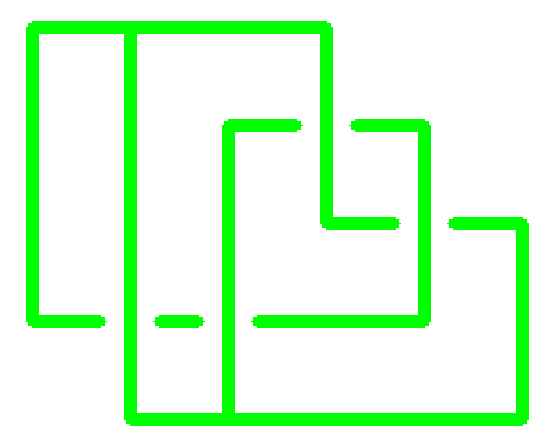
\includegraphics[width=1.25cm]{../Midterm_Poster/grid_diagram/theta_3_1.png}
    \caption{$3_1$} 
    \end{subfigure}
    \begin{subfigure}{0.075\textwidth}
    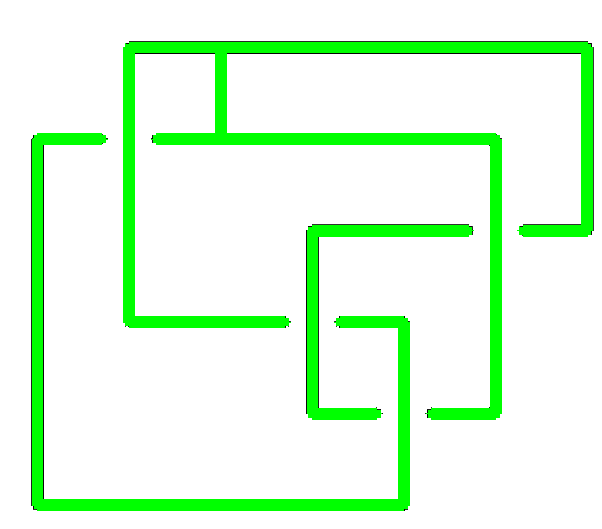
\includegraphics[width=1.25cm]{../Midterm_Poster/grid_diagram/theta_4_1.png}
    \caption{$4_1$} 
    \end{subfigure}
    \begin{subfigure}{0.075\textwidth}
    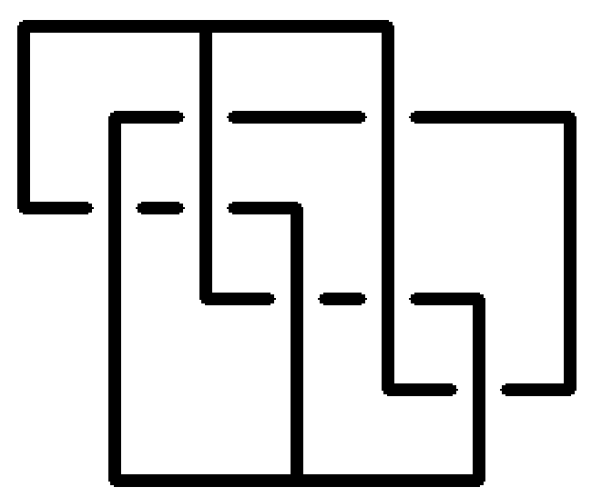
\includegraphics[width=1.25cm]{../Midterm_Poster/grid_diagram/theta_5_1.png}
    \caption{$5_1$}
    \end{subfigure}
    \begin{subfigure}{0.075\textwidth}
    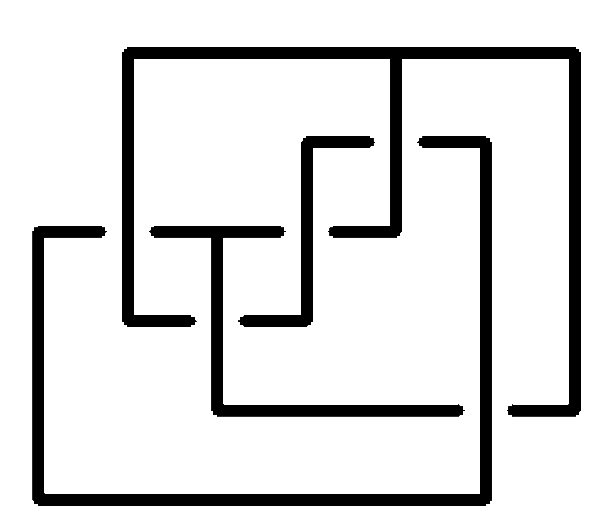
\includegraphics[width=1.25cm]{../Midterm_Poster/grid_diagram/theta_5_2.png}
    \caption{$5_2$} 
    \end{subfigure}
    \begin{subfigure}{0.075\textwidth}
    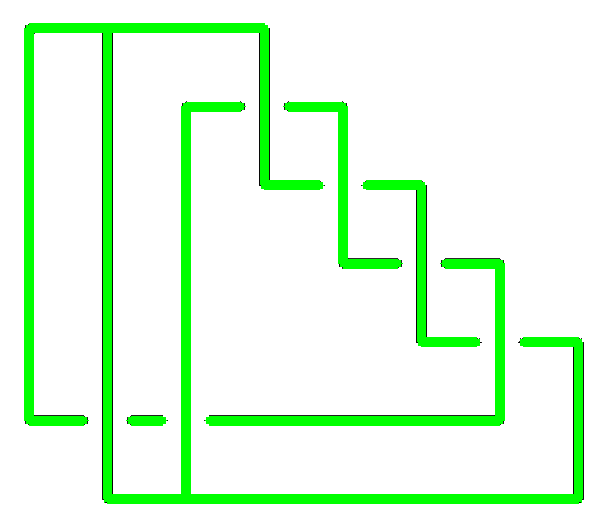
\includegraphics[width=1.25cm]{../Midterm_Poster/grid_diagram/theta_5_3.png}
    \caption{$5_3$}
    \end{subfigure}
    \begin{subfigure}{0.075\textwidth}
    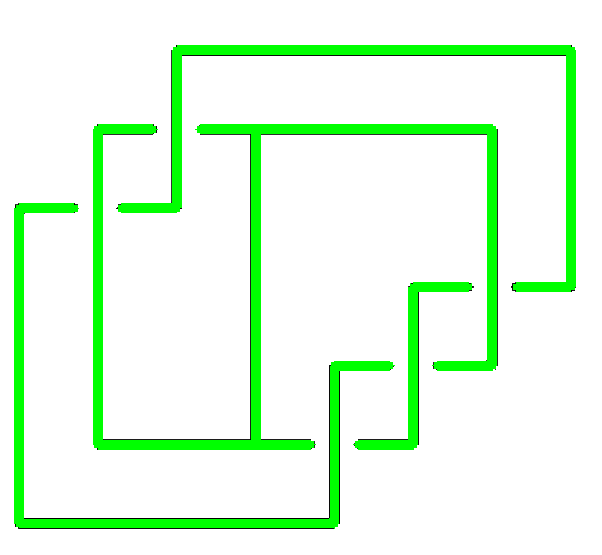
\includegraphics[width=1.25cm]{../Midterm_Poster/grid_diagram/theta_5_4.png}
    \caption{$5_4$} 
    \end{subfigure}
    \begin{subfigure}{0.075\textwidth}
    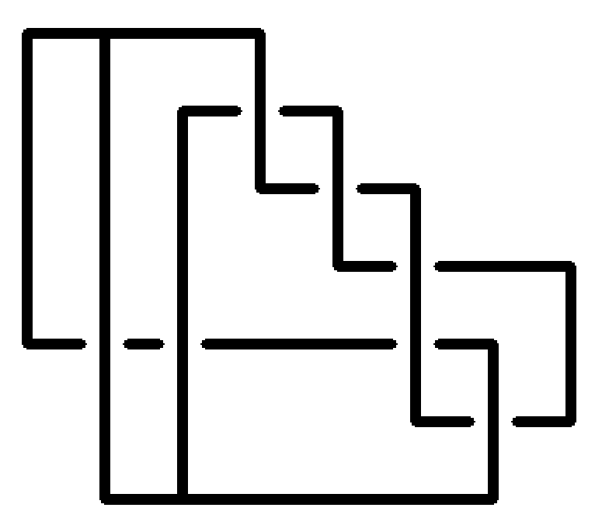
\includegraphics[width=1.25cm]{../Midterm_Poster/grid_diagram/theta_5_5.png}
    \caption{$5_5$} 
    \end{subfigure}
    \begin{subfigure}{0.075\textwidth}
    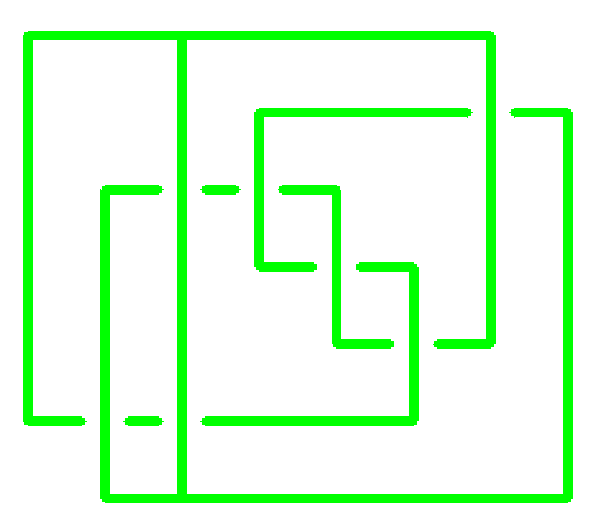
\includegraphics[width=1.25cm]{../Midterm_Poster/grid_diagram/theta_5_6.png}
    \caption{$5_6$} 
    \end{subfigure}
    \begin{subfigure}{0.075\textwidth}
    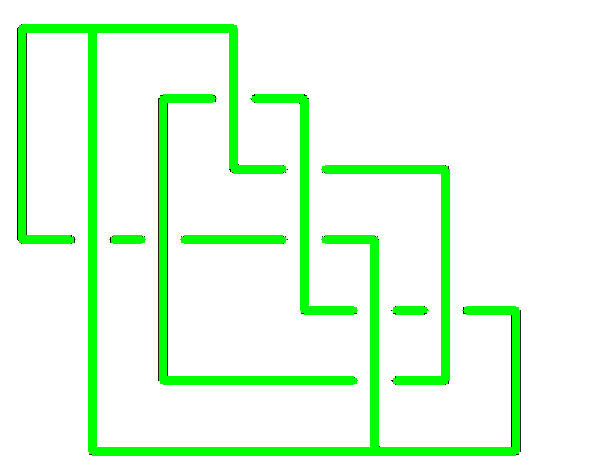
\includegraphics[width=1.25cm]{../Midterm_Poster/grid_diagram/theta_5_7.png}
    \caption{$5_7$} 
    \end{subfigure}
    \begin{subfigure}{0.075\textwidth}
    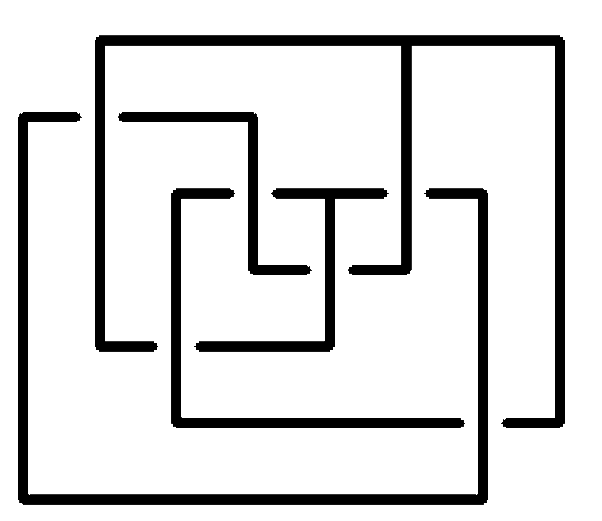
\includegraphics[width=1.25cm]{../Midterm_Poster/grid_diagram/theta_6_1.png}
    \caption{$6_1$} 
    \end{subfigure}
    \begin{subfigure}{0.075\textwidth}
    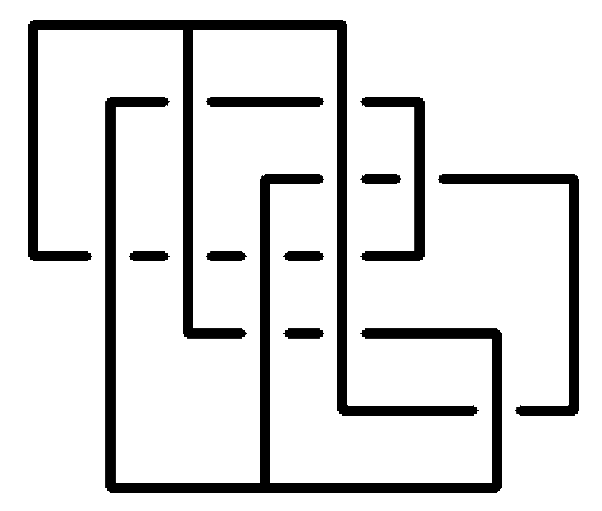
\includegraphics[width=1.25cm]{../Midterm_Poster/grid_diagram/theta_6_2.png}
    \caption{$6_2$} 
    \end{subfigure}
    \begin{subfigure}{0.075\textwidth}
    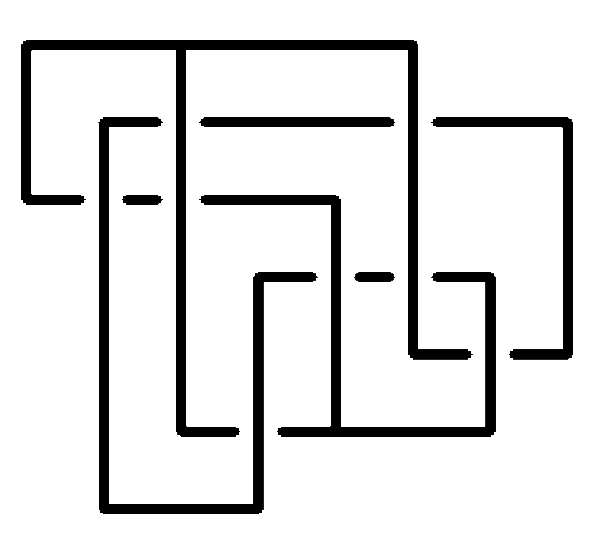
\includegraphics[width=1.25cm]{../Midterm_Poster/grid_diagram/theta_6_3.png}
    \caption{$6_3$} 
    \end{subfigure}
    \begin{subfigure}{0.075\textwidth}
    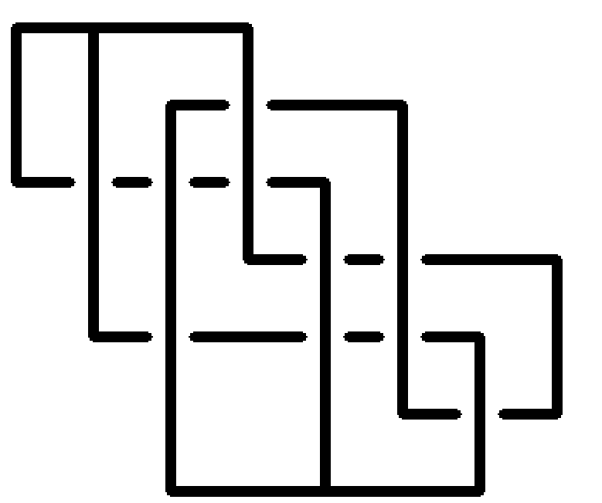
\includegraphics[width=1.25cm]{../Midterm_Poster/grid_diagram/theta_6_4.png}
    \caption{$6_4$} 
    \end{subfigure}
    \begin{subfigure}{0.075\textwidth}
    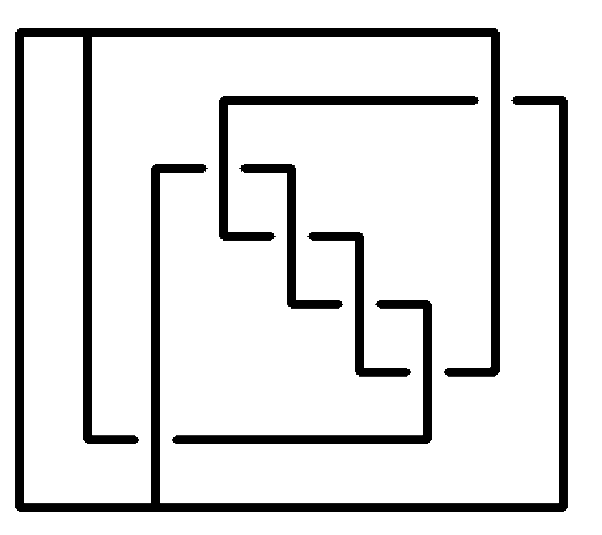
\includegraphics[width=1.25cm]{../Midterm_Poster/grid_diagram/theta_6_5.png}
    \caption{$6_5$} 
    \end{subfigure}
    \begin{subfigure}{0.075\textwidth}
    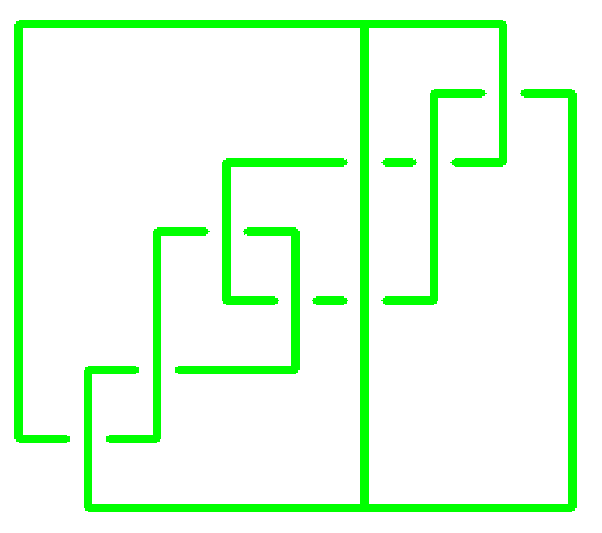
\includegraphics[width=1.25cm]{../Midterm_Poster/grid_diagram/theta_6_6.png}
    \caption{$6_6$} 
    \end{subfigure}
    \begin{subfigure}{0.075\textwidth}
    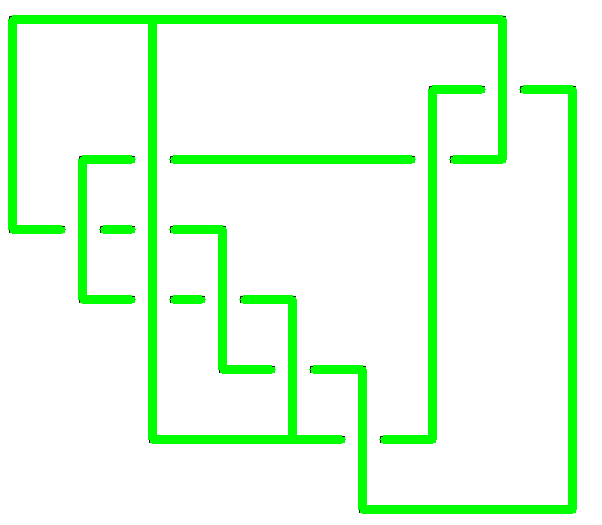
\includegraphics[width=1.25cm]{../Midterm_Poster/grid_diagram/theta_6_7.png}
    \caption{$6_7$} 
    \end{subfigure}
      \begin{subfigure}{0.075\textwidth}
    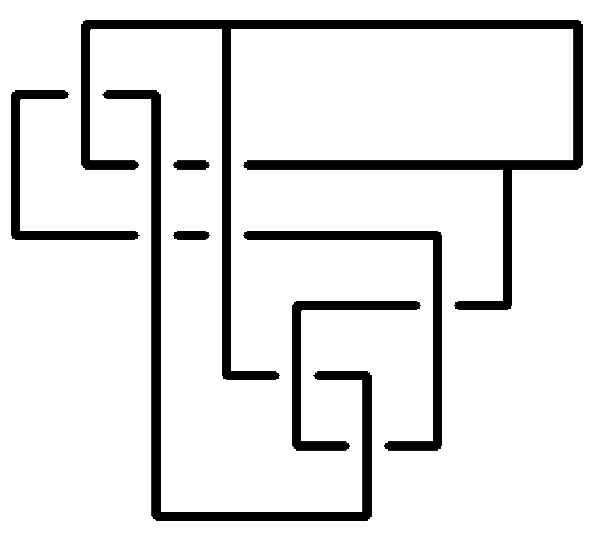
\includegraphics[width=1.25cm]{../Midterm_Poster/grid_diagram/theta_6_8.png}
    \caption{$6_8$} 
    \end{subfigure}
    \begin{subfigure}{0.075\textwidth}
    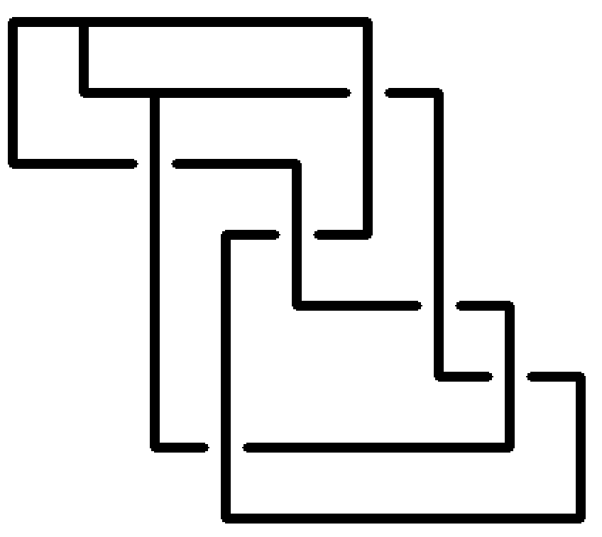
\includegraphics[width=1.25cm]{../Midterm_Poster/grid_diagram/theta_6_9.png}
    \caption{$6_9$} 
    \end{subfigure}
    \begin{subfigure}{0.075\textwidth}
    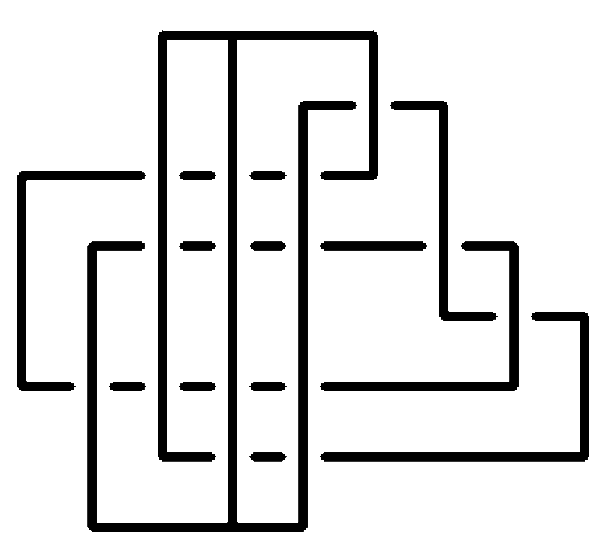
\includegraphics[width=1.25cm]{../Midterm_Poster/grid_diagram/theta_6_10.png}
    \caption{$6_{10}$} 
    \end{subfigure}
    \begin{subfigure}{0.075\textwidth}
    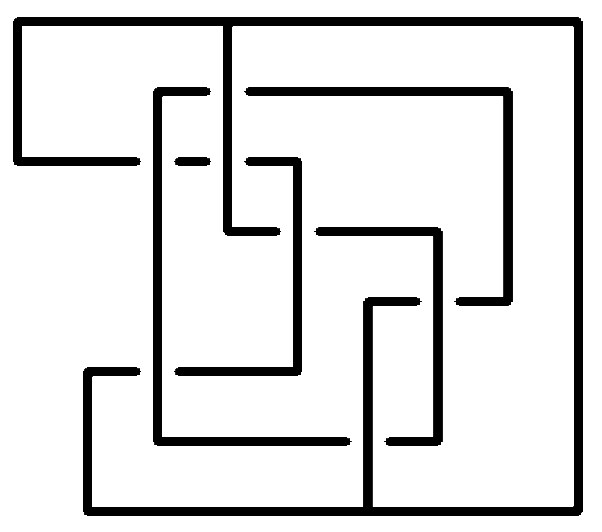
\includegraphics[width=1.25cm]{../Midterm_Poster/grid_diagram/theta_6_11.png}
    \caption{$6_{11}$} 
    \end{subfigure}
    \begin{subfigure}{0.075\textwidth}
    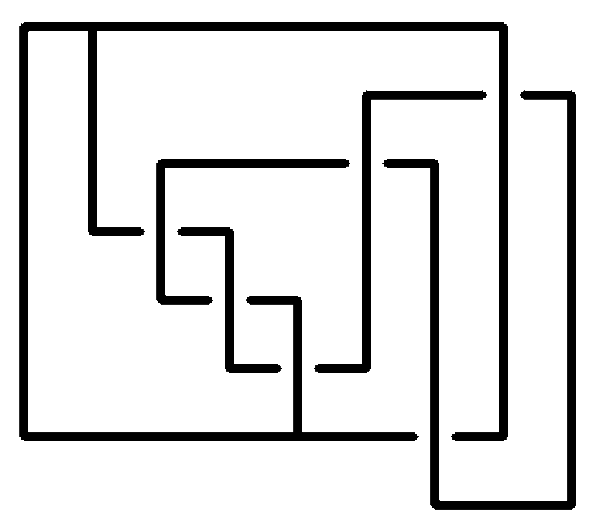
\includegraphics[width=1.25cm]{../Midterm_Poster/grid_diagram/theta_6_12.png}
    \caption{$6_{12}$} 
    \end{subfigure}
    \begin{subfigure}{0.075\textwidth}
    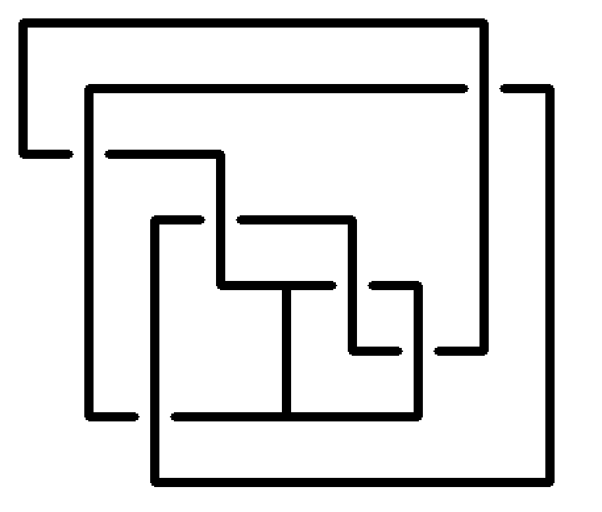
\includegraphics[width=1.25cm]{../Midterm_Poster/grid_diagram/theta_6_13.png}
    \caption{$6_{13}$} 
    \end{subfigure}
    \begin{subfigure}{0.075\textwidth}
    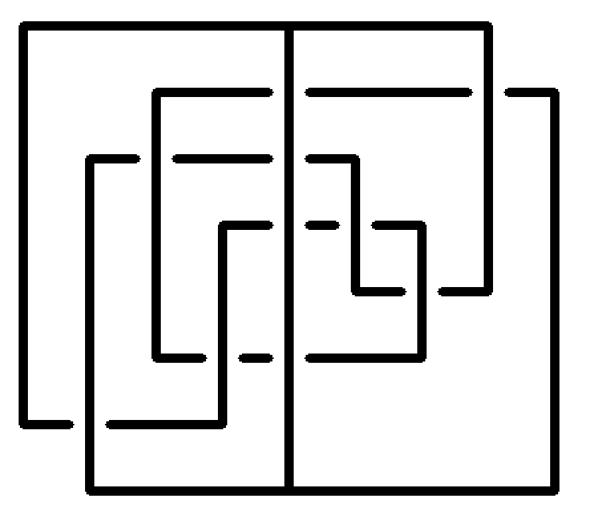
\includegraphics[width=1.25cm]{../Midterm_Poster/grid_diagram/theta_6_14.png}
    \caption{$6_{14}$} 
    \end{subfigure}
    \begin{subfigure}{0.075\textwidth}
    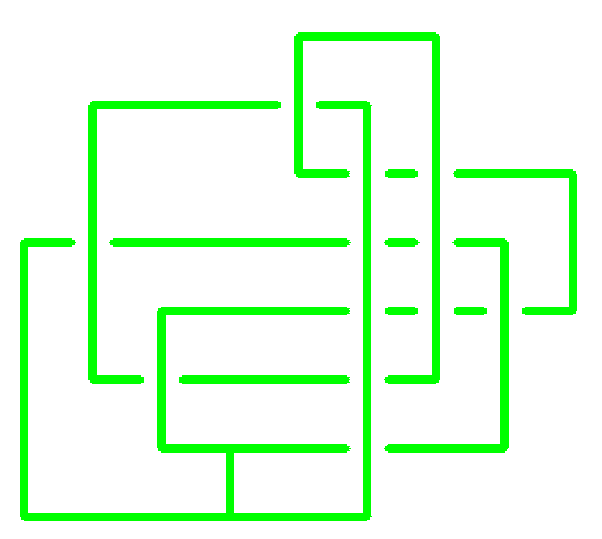
\includegraphics[width=1.25cm]{../Midterm_Poster/grid_diagram/theta_6_15.png}
    \caption{$6_{15}$} 
    \end{subfigure}
    \begin{subfigure}{0.075\textwidth}
    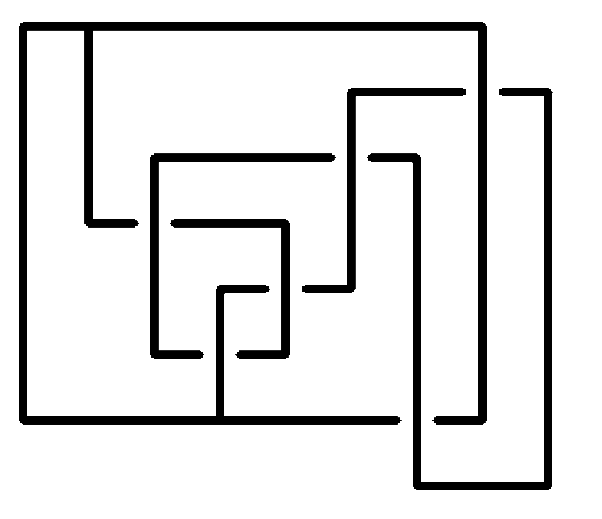
\includegraphics[width=1.25cm]{../Midterm_Poster/grid_diagram/theta_6_16.png}
    \caption{$6_{16}$} 
    \end{subfigure}
    \begin{subfigure}{0.075\textwidth}
    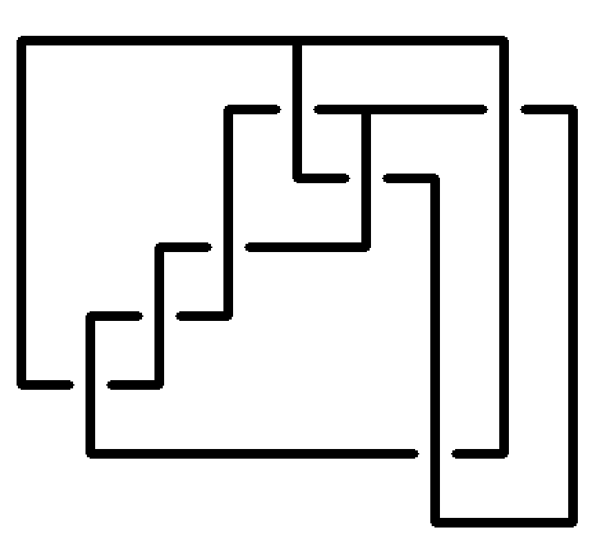
\includegraphics[width=1.25cm]{../Midterm_Poster/grid_diagram/theta_7_1.png}
    \caption{$7_{1}$} 
    \end{subfigure}
    \begin{subfigure}{0.075\textwidth}
    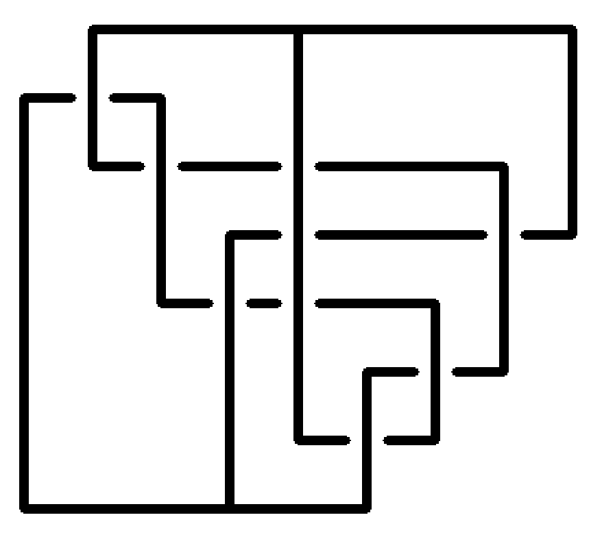
\includegraphics[width=1.25cm]{../Midterm_Poster/grid_diagram/theta_7_2.png}
    \caption{$7_{2}$} 
    \end{subfigure}
    \begin{subfigure}{0.075\textwidth}
    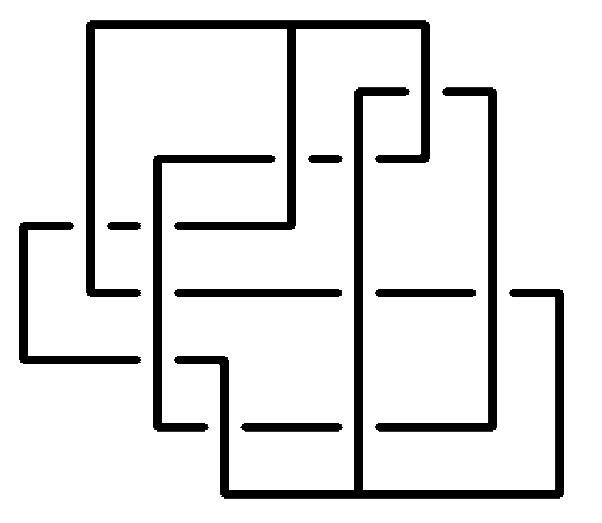
\includegraphics[width=1.25cm]{../Midterm_Poster/grid_diagram/theta_7_3.png}
    \caption{$7_{3}$} 
    \end{subfigure}
    \begin{subfigure}{0.075\textwidth}
    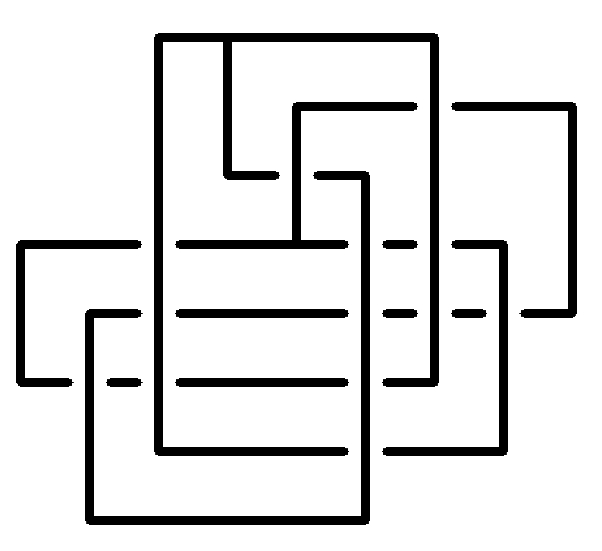
\includegraphics[width=1.25cm]{../Midterm_Poster/grid_diagram/theta_7_4.png}
    \caption{$7_{4}$} 
    \end{subfigure}
    \begin{subfigure}{0.075\textwidth}
    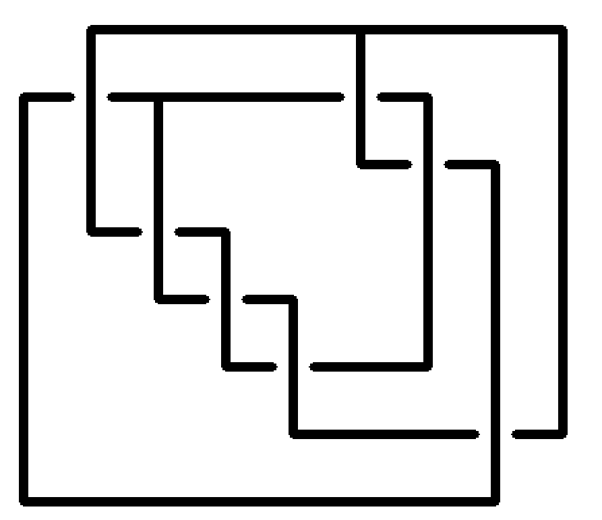
\includegraphics[width=1.25cm]{../Midterm_Poster/grid_diagram/theta_7_5.png}
    \caption{$7_{5}$} 
    \end{subfigure}
    \begin{subfigure}{0.075\textwidth}
    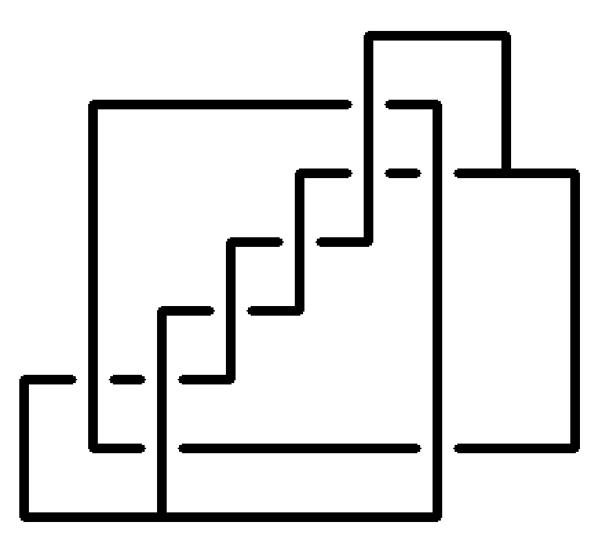
\includegraphics[width=1.25cm]{../Midterm_Poster/grid_diagram/theta_7_6.png}
    \caption{$7_{6}$} 
    \end{subfigure}
    \begin{subfigure}{0.075\textwidth}
    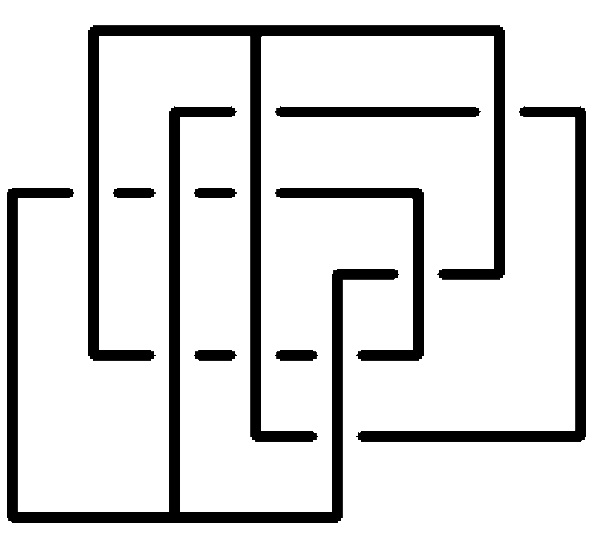
\includegraphics[width=1.25cm]{../Midterm_Poster/grid_diagram/theta_7_7.png}
    \caption{$7_{7}$} 
    \end{subfigure}
    \begin{subfigure}{0.075\textwidth}
    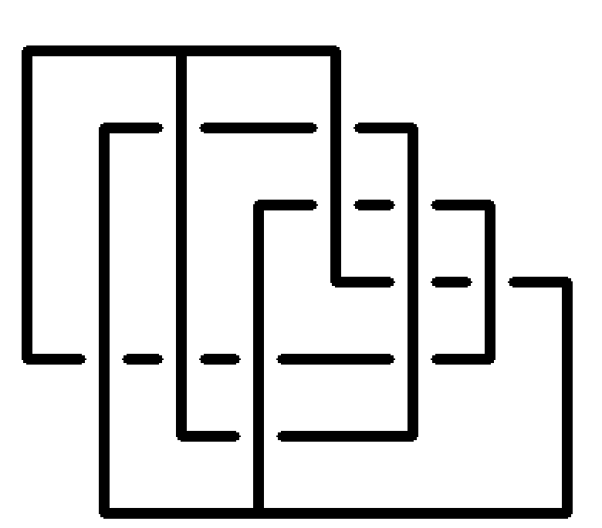
\includegraphics[width=1.25cm]{../Midterm_Poster/grid_diagram/theta_7_8.png}
    \caption{$7_{8}$} 
    \end{subfigure}
    \begin{subfigure}{0.075\textwidth}
    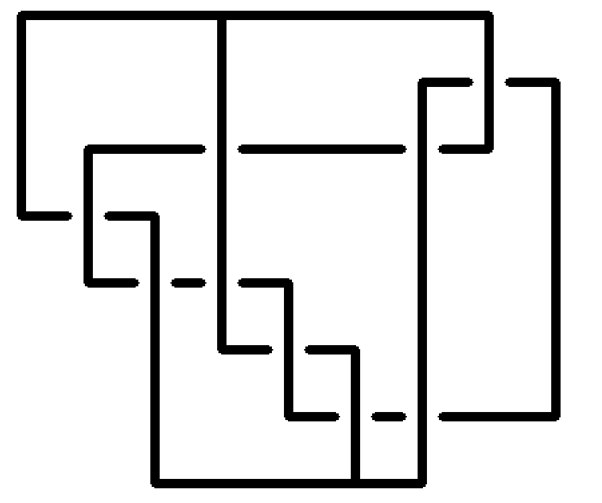
\includegraphics[width=1.25cm]{../Midterm_Poster/grid_diagram/theta_7_9.png}
    \caption{$7_{9}$} 
    \end{subfigure}
    \begin{subfigure}{0.075\textwidth}
    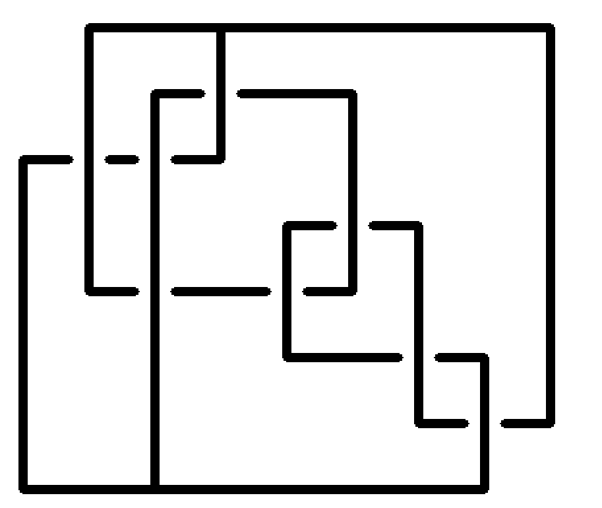
\includegraphics[width=1.25cm]{../Midterm_Poster/grid_diagram/theta_7_10.png}
    \caption{$7_{10}$} 
    \end{subfigure}
    \begin{subfigure}{0.075\textwidth}
    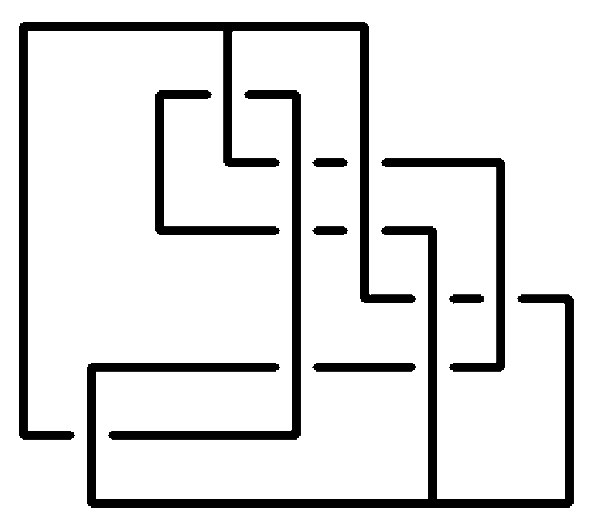
\includegraphics[width=1.25cm]{../Midterm_Poster/grid_diagram/theta_7_11.png}
    \caption{$7_{11}$} 
    \end{subfigure}
    \begin{subfigure}{0.075\textwidth}
    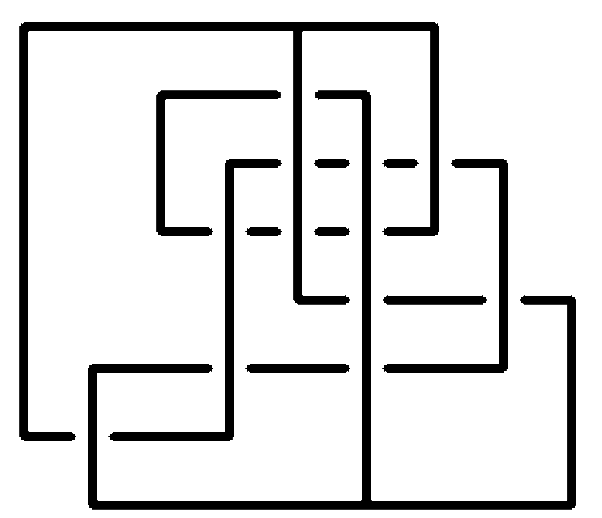
\includegraphics[width=1.25cm]{../Midterm_Poster/grid_diagram/theta_7_12.png}
    \caption{$7_{12}$} 
    \end{subfigure}
    \begin{subfigure}{0.075\textwidth}
    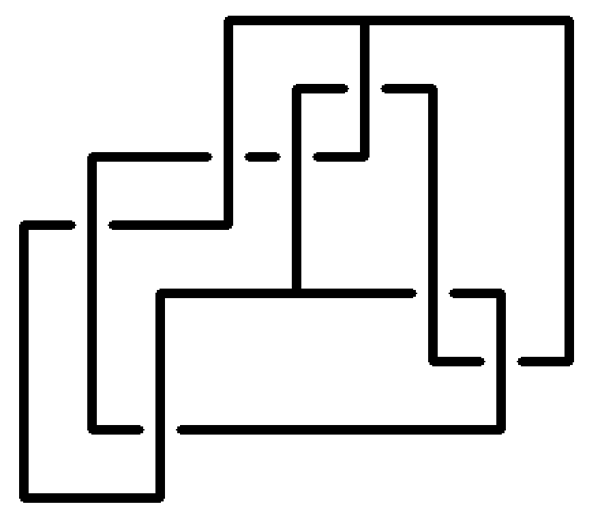
\includegraphics[width=1.25cm]{../Midterm_Poster/grid_diagram/theta_7_13.png}
    \caption{$7_{13}$} 
    \end{subfigure}
    \begin{subfigure}{0.075\textwidth}
    \includegraphics[width=1.25cm]{../Midterm_Poster/grid_diagram/theta_7_14.png}
    \caption{$7_{14}$} 
    \end{subfigure}
    \begin{subfigure}{0.075\textwidth}
    \includegraphics[width=1.25cm]{../Midterm_Poster/grid_diagram/theta_7_15.png}
    \caption{$7_{15}$} 
    \end{subfigure}
    \begin{subfigure}{0.075\textwidth}
    \includegraphics[width=1.25cm]{../Midterm_Poster/grid_diagram/theta_7_16.png}
    \caption{$7_{16}$} 
    \end{subfigure}
    \begin{subfigure}{0.075\textwidth}
    \includegraphics[width=1.25cm]{../Midterm_Poster/grid_diagram/theta_7_17.png}
    \caption{$7_{17}$} 
    \end{subfigure}
    \begin{subfigure}{0.075\textwidth}
    \includegraphics[width=1.25cm]{../Midterm_Poster/grid_diagram/theta_7_18.png}
    \caption{$7_{18}$} 
    \end{subfigure}
    \begin{subfigure}{0.075\textwidth}
    \includegraphics[width=1.25cm]{../Midterm_Poster/grid_diagram/theta_7_19.png}
    \caption{$7_{19}$} 
    \end{subfigure}
    \begin{subfigure}{0.075\textwidth}
    \includegraphics[width=1.25cm]{../Midterm_Poster/grid_diagram/theta_7_20.png}
    \caption{$7_{20}$} 
    \end{subfigure}
    \begin{subfigure}{0.075\textwidth}
    \includegraphics[width=1.25cm]{../Midterm_Poster/grid_diagram/theta_7_21.png}
    \caption{$7_{21}$} 
    \end{subfigure}
    \begin{subfigure}{0.075\textwidth}
    \includegraphics[width=1.25cm]{../Midterm_Poster/grid_diagram/theta_7_22.png}
    \caption{$7_{22}$} 
    \end{subfigure}
    \begin{subfigure}{0.075\textwidth}
    \includegraphics[width=1.25cm]{../Midterm_Poster/grid_diagram/theta_7_23.png}
    \caption{$7_{23}$} 
    \end{subfigure}
    \begin{subfigure}{0.075\textwidth}
    \includegraphics[width=1.25cm]{../Midterm_Poster/grid_diagram/theta_7_24.png}
    \caption{$7_{24}$} 
    \end{subfigure}
    \begin{subfigure}{0.075\textwidth}
    \includegraphics[width=1.25cm]{../Midterm_Poster/grid_diagram/theta_7_25.png}
    \caption{$7_{25}$} 
    \end{subfigure}
    \begin{subfigure}{0.075\textwidth}
    \includegraphics[width=1.25cm]{../Midterm_Poster/grid_diagram/theta_7_26.png}
    \caption{$7_{26}$} 
    \end{subfigure}
    \begin{subfigure}{0.075\textwidth}
    \includegraphics[width=1.25cm]{../Midterm_Poster/grid_diagram/theta_7_27.png}
    \caption{$7_{27}$} 
    \end{subfigure}
    \begin{subfigure}{0.075\textwidth}
    \includegraphics[width=1.25cm]{../Midterm_Poster/grid_diagram/theta_7_28.png}
    \caption{$7_{28}$} 
    \end{subfigure}
    \begin{subfigure}{0.075\textwidth}
    \includegraphics[width=1.25cm]{../Midterm_Poster/grid_diagram/theta_7_29.png}
    \caption{$7_{29}$} 
    \end{subfigure}
    \begin{subfigure}{0.075\textwidth}
    \includegraphics[width=1.25cm]{../Midterm_Poster/grid_diagram/theta_7_30.png}
    \caption{$7_{30}$}
    \end{subfigure}
    \begin{subfigure}{0.075\textwidth}
    \includegraphics[width=1.25cm]{../Midterm_Poster/grid_diagram/theta_7_31.png}
    \caption{$7_{31}$} 
    \end{subfigure}
    \begin{subfigure}{0.075\textwidth}
    \includegraphics[width=1.25cm]{../Midterm_Poster/grid_diagram/theta_7_32.png}
    \caption{$7_{32}$} 
    \end{subfigure}
    \begin{subfigure}{0.075\textwidth}
    \includegraphics[width=1.25cm]{../Midterm_Poster/grid_diagram/theta_7_33.png}
    \caption{$7_{33}$} 
    \end{subfigure}
    \begin{subfigure}{0.075\textwidth}
    \includegraphics[width=1.25cm]{../Midterm_Poster/grid_diagram/theta_7_34.png}
    \caption{$7_{34}$} 
    \end{subfigure}
    \begin{subfigure}{0.075\textwidth}
    \includegraphics[width=1.25cm]{../Midterm_Poster/grid_diagram/theta_7_35.png}
    \caption{$7_{35}$} 
    \end{subfigure}
    \begin{subfigure}{0.075\textwidth}
    \includegraphics[width=1.25cm]{../Midterm_Poster/grid_diagram/theta_7_36.png}
    \caption{$7_{36}$} 
    \end{subfigure}
    \begin{subfigure}{0.075\textwidth}
    \includegraphics[width=1.25cm]{../Midterm_Poster/grid_diagram/theta_7_37.png}
    \caption{$7_{37}$} 
    \end{subfigure}
    \begin{subfigure}{0.075\textwidth}
    \includegraphics[width=1.25cm]{../Midterm_Poster/grid_diagram/theta_7_38.png}
    \caption{$7_{38}$} 
    \end{subfigure}
    \begin{subfigure}{0.075\textwidth}
    \includegraphics[width=1.25cm]{../Midterm_Poster/grid_diagram/theta_7_39.png}
    \caption{$7_{39}$} 
    \end{subfigure}
    \begin{subfigure}{0.075\textwidth}
    \includegraphics[width=1.25cm]{../Midterm_Poster/grid_diagram/theta_7_40.png}
    \caption{$7_{40}$} 
    \end{subfigure}
    \begin{subfigure}{0.075\textwidth}
    \includegraphics[width=1.25cm]{../Midterm_Poster/grid_diagram/theta_7_41.png}
    \caption{$7_{41}$} 
    \end{subfigure}
    \begin{subfigure}{0.075\textwidth}
    \includegraphics[width=1.25cm]{../Midterm_Poster/grid_diagram/theta_7_42.png}
    \caption{$7_{42}$} 
    \end{subfigure}
    \begin{subfigure}{0.075\textwidth}
    \includegraphics[width=1.25cm]{../Midterm_Poster/grid_diagram/theta_7_43.png}
    \caption{$7_{43}$} 
    \end{subfigure}
    \begin{subfigure}{0.075\textwidth}
    \includegraphics[width=1.25cm]{../Midterm_Poster/grid_diagram/theta_7_44.png}
    \caption{$7_{44}$} 
    \end{subfigure}
    \begin{subfigure}{0.075\textwidth}
    \includegraphics[width=1.25cm]{../Midterm_Poster/grid_diagram/theta_7_45.png}
    \caption{$7_{45}$} 
    \end{subfigure}
    \begin{subfigure}{0.075\textwidth}
    \includegraphics[width=1.25cm]{../Midterm_Poster/grid_diagram/theta_7_46.png}
    \caption{$7_{46}$} 
    \end{subfigure}
    \begin{subfigure}{0.075\textwidth}
    \includegraphics[width=1.25cm]{../Midterm_Poster/grid_diagram/theta_7_47.png}
    \caption{$7_{47}$} 
    \end{subfigure}
    \begin{subfigure}{0.075\textwidth}
    \includegraphics[width=1.25cm]{../Midterm_Poster/grid_diagram/theta_7_48.png}
    \caption{$7_{48}$} 
    \end{subfigure}
    \begin{subfigure}{0.075\textwidth}
    \includegraphics[width=1.25cm]{../Midterm_Poster/grid_diagram/theta_7_49.png}
    \caption{$7_{49}$} 
    \end{subfigure}
    \begin{subfigure}{0.075\textwidth}
    \includegraphics[width=1.25cm]{../Midterm_Poster/grid_diagram/theta_7_50.png}
    \caption{$7_{50}$} 
    \end{subfigure}
    \begin{subfigure}{0.075\textwidth}
    \includegraphics[width=1.25cm]{../Midterm_Poster/grid_diagram/theta_7_51.png}
    \caption{$7_{51}$} 
    \end{subfigure}
    \begin{subfigure}{0.075\textwidth}
    \includegraphics[width=1.25cm]{../Midterm_Poster/grid_diagram/theta_7_52.png}
    \caption{$7_{52}$} 
    \end{subfigure}
    \begin{subfigure}{0.075\textwidth}
    \includegraphics[width=1.25cm]{../Midterm_Poster/grid_diagram/theta_7_53.png}
    \caption{$7_{53}$} 
    \end{subfigure}
    \begin{subfigure}{0.075\textwidth}
    \includegraphics[width=1.25cm]{../Midterm_Poster/grid_diagram/theta_7_54.png}
    \caption{$7_{54}$} 
    \end{subfigure}
    \begin{subfigure}{0.075\textwidth}
    \includegraphics[width=1.25cm]{../Midterm_Poster/grid_diagram/theta_7_55.png}
    \caption{$7_{55}$} 
    \end{subfigure}
    \begin{subfigure}{0.075\textwidth}
    \includegraphics[width=1.25cm]{../Midterm_Poster/grid_diagram/theta_7_56.png}
    \caption{$7_{56}$} 
    \end{subfigure}
    \begin{subfigure}{0.075\textwidth}
    \includegraphics[width=1.25cm]{../Midterm_Poster/grid_diagram/theta_7_57.png}
    \caption{$7_{57}$} 
    \end{subfigure}
    \begin{subfigure}{0.075\textwidth}
    \includegraphics[width=1.25cm]{../Midterm_Poster/grid_diagram/theta_7_58.png}
    \caption{$7_{58}$} 
    \end{subfigure}
    \begin{subfigure}{0.075\textwidth}
    \includegraphics[width=1.25cm]{../Midterm_Poster/grid_diagram/theta_7_59.png}
    \caption{$7_{59}$} 
    \end{subfigure}
    \begin{subfigure}{0.075\textwidth}
    \includegraphics[width=1.25cm]{../Midterm_Poster/grid_diagram/theta_7_60.png}
    \caption{$7_{60}$} 
    \end{subfigure}
    \begin{subfigure}{0.075\textwidth}
    \includegraphics[width=1.25cm]{../Midterm_Poster/grid_diagram/theta_7_61.png}
    \caption{$7_{61}$} 
    \end{subfigure}
    \begin{subfigure}{0.075\textwidth}
    \includegraphics[width=1.25cm]{../Midterm_Poster/grid_diagram/theta_7_62.png}
    \caption{$7_{62}$} 
    \end{subfigure}
    \begin{subfigure}{0.075\textwidth}
    \includegraphics[width=1.25cm]{../Midterm_Poster/grid_diagram/theta_7_63.png}
    \caption{$7_{63}$} 
    \end{subfigure}
    \begin{subfigure}{0.075\textwidth}
    \includegraphics[width=1.25cm]{../Midterm_Poster/grid_diagram/theta_7_64.png}
    \caption{$7_{64}$} 
    \end{subfigure}
    \begin{subfigure}{0.075\textwidth}
    \includegraphics[width=1.25cm]{../Midterm_Poster/grid_diagram/theta_7_65.png}
    \caption{$7_{65}$} 
    \end{subfigure}
    \caption{Grid Diagram of the Theta-Curves Up to 7 Crossings}
  \end{figure}

  \begin{figure}[H]
    \begin{subfigure}{0.075\textwidth}
    \includegraphics[width=1.25cm]{../Midterm_Poster/grid_diagram/handcuff_2_1.png}
    \caption{$2_{1}$} 
    \end{subfigure}
    \begin{subfigure}{0.075\textwidth}
    \includegraphics[width=1.25cm]{../Midterm_Poster/grid_diagram/handcuff_4_1.png}
    \caption{$4_{1}$} 
    \end{subfigure}
    \begin{subfigure}{0.075\textwidth}
    \includegraphics[width=1.25cm]{../Midterm_Poster/grid_diagram/handcuff_5_1.png}
    \caption{$5_{1}$} 
    \end{subfigure}
    \begin{subfigure}{0.075\textwidth}
    \includegraphics[width=1.25cm]{../Midterm_Poster/grid_diagram/handcuff_6_1.png}
    \caption{$6_{1}$} 
    \end{subfigure}
    \begin{subfigure}{0.075\textwidth}
    \includegraphics[width=1.25cm]{../Midterm_Poster/grid_diagram/handcuff_6_2.png}
    \caption{$6_{2}$} 
    \end{subfigure}
    \begin{subfigure}{0.075\textwidth}
    \includegraphics[width=1.25cm]{../Midterm_Poster/grid_diagram/handcuff_6_3.png}
    \caption{$6_{3}$} 
    \end{subfigure}
    \begin{subfigure}{0.075\textwidth}
    \includegraphics[width=1.25cm]{../Midterm_Poster/grid_diagram/handcuff_6_4.png}
    \caption{$6_{4}$} 
    \end{subfigure}
    \begin{subfigure}{0.075\textwidth}
    \includegraphics[width=1.25cm]{../Midterm_Poster/grid_diagram/handcuff_6_5.png}
    \caption{$6_{5}$} 
    \end{subfigure}
    \begin{subfigure}{0.075\textwidth}
    \includegraphics[width=1.25cm]{../Midterm_Poster/grid_diagram/handcuff_6_6.png}
    \caption{$6_{6}$} 
    \end{subfigure}
    \begin{subfigure}{0.075\textwidth}
    \includegraphics[width=1.25cm]{../Midterm_Poster/grid_diagram/handcuff_6_7.png}
    \caption{$6_{7}$} 
    \end{subfigure}
    \begin{subfigure}{0.075\textwidth}
    \includegraphics[width=1.25cm]{../Midterm_Poster/grid_diagram/handcuff_6_8.png}
    \caption{$6_{8}$} 
    \end{subfigure}
    \begin{subfigure}{0.075\textwidth}
    \includegraphics[width=1.25cm]{../Midterm_Poster/grid_diagram/handcuff_6_9.png}
    \caption{$6_{9}$} 
    \end{subfigure}
    \begin{subfigure}{0.075\textwidth}
    \includegraphics[width=1.25cm]{../Midterm_Poster/grid_diagram/handcuff_7_1.png}
    \caption{$7_{1}$} 
    \end{subfigure}
    \begin{subfigure}{0.075\textwidth}
    \includegraphics[width=1.25cm]{../Midterm_Poster/grid_diagram/handcuff_7_2.png}
    \caption{$7_{2}$} 
    \end{subfigure}
    \begin{subfigure}{0.075\textwidth}
    \includegraphics[width=1.25cm]{../Midterm_Poster/grid_diagram/handcuff_7_3.png}
    \caption{$7_{3}$} 
    \end{subfigure}
    \begin{subfigure}{0.075\textwidth}
    \includegraphics[width=1.25cm]{../Midterm_Poster/grid_diagram/handcuff_7_4.png}
    \caption{$7_{4}$} 
    \end{subfigure}
    \begin{subfigure}{0.075\textwidth}
    \includegraphics[width=1.25cm]{../Midterm_Poster/grid_diagram/handcuff_7_5.png}
    \caption{$7_{5}$} 
    \end{subfigure}
    \begin{subfigure}{0.075\textwidth}
    \includegraphics[width=1.25cm]{../Midterm_Poster/grid_diagram/handcuff_7_6.png}
    \caption{$7_{6}$} 
    \end{subfigure}
    \begin{subfigure}{0.075\textwidth}
    \includegraphics[width=1.25cm]{../Midterm_Poster/grid_diagram/handcuff_7_7.png}
    \caption{$7_{7}$} 
    \end{subfigure}
    \begin{subfigure}{0.075\textwidth}
    \includegraphics[width=1.25cm]{../Midterm_Poster/grid_diagram/handcuff_7_8.png}
    \caption{$7_{8}$} 
    \end{subfigure}
    \begin{subfigure}{0.075\textwidth}
    \includegraphics[width=1.25cm]{../Midterm_Poster/grid_diagram/handcuff_7_9.png}
    \caption{$7_{9}$} 
    \end{subfigure}
    \begin{subfigure}{0.075\textwidth}
    \includegraphics[width=1.25cm]{../Midterm_Poster/grid_diagram/handcuff_7_10.png}
    \caption{$7_{10}$} 
    \end{subfigure}
    \begin{subfigure}{0.075\textwidth}
    \includegraphics[width=1.25cm]{../Midterm_Poster/grid_diagram/handcuff_7_11.png}
    \caption{$7_{11}$} 
    \end{subfigure}
    \begin{subfigure}{0.075\textwidth}
    \includegraphics[width=1.25cm]{../Midterm_Poster/grid_diagram/handcuff_7_12.png}
    \caption{$7_{12}$} 
    \end{subfigure}
    \begin{subfigure}{0.075\textwidth}
    \includegraphics[width=1.25cm]{../Midterm_Poster/grid_diagram/handcuff_7_13.png}
    \caption{$7_{13}$} 
    \end{subfigure}
    \begin{subfigure}{0.075\textwidth}
    \includegraphics[width=1.25cm]{../Midterm_Poster/grid_diagram/handcuff_7_14.png}
    \caption{$7_{14}$} 
    \end{subfigure}
    \begin{subfigure}{0.075\textwidth}
    \includegraphics[width=1.25cm]{../Midterm_Poster/grid_diagram/handcuff_7_15.png}
    \caption{$7_{15}$} 
    \end{subfigure}
    \begin{subfigure}{0.075\textwidth}
    \includegraphics[width=1.25cm]{../Midterm_Poster/grid_diagram/handcuff_7_16.png}
    \caption{$7_{16}$} 
    \end{subfigure}
    \begin{subfigure}{0.075\textwidth}
    \includegraphics[width=1.25cm]{../Midterm_Poster/grid_diagram/handcuff_7_17.png}
    \caption{$7_{17}$} 
    \end{subfigure}
    \begin{subfigure}{0.075\textwidth}
    \includegraphics[width=1.25cm]{../Midterm_Poster/grid_diagram/handcuff_7_18.png}
    \caption{$7_{18}$} 
    \end{subfigure}
    \begin{subfigure}{0.075\textwidth}
    \includegraphics[width=1.25cm]{../Midterm_Poster/grid_diagram/handcuff_7_19.png}
    \caption{$7_{19}$} 
    \end{subfigure}
    \begin{subfigure}{0.075\textwidth}
    \includegraphics[width=1.25cm]{../Midterm_Poster/grid_diagram/handcuff_7_20.png}
    \caption{$7_{20}$} 
    \end{subfigure}
    \begin{subfigure}{0.075\textwidth}
    \includegraphics[width=1.25cm]{../Midterm_Poster/grid_diagram/handcuff_7_21.png}
    \caption{$7_{21}$} 
    \end{subfigure}
    \begin{subfigure}{0.075\textwidth}
    \includegraphics[width=1.25cm]{../Midterm_Poster/grid_diagram/handcuff_7_22.png}
    \caption{$7_{22}$} 
    \end{subfigure}
    \begin{subfigure}{0.075\textwidth}
    \includegraphics[width=1.25cm]{../Midterm_Poster/grid_diagram/handcuff_7_23.png}
    \caption{$7_{23}$} 
    \end{subfigure}
    \begin{subfigure}{0.075\textwidth}
    \includegraphics[width=1.25cm]{../Midterm_Poster/grid_diagram/handcuff_7_24.png}
    \caption{$7_{24}$} 
    \end{subfigure}
    \begin{subfigure}{0.075\textwidth}
    \includegraphics[width=1.25cm]{../Midterm_Poster/grid_diagram/handcuff_7_25.png}
    \caption{$7_{25}$} 
    \end{subfigure}
    \begin{subfigure}{0.075\textwidth}
    \includegraphics[width=1.25cm]{../Midterm_Poster/grid_diagram/handcuff_7_26.png}
    \caption{$7_{26}$} 
    \end{subfigure}
    \begin{subfigure}{0.075\textwidth}
    \includegraphics[width=1.25cm]{../Midterm_Poster/grid_diagram/handcuff_7_27.png}
    \caption{$7_{27}$} 
    \end{subfigure}
    \begin{subfigure}{0.075\textwidth}
    \includegraphics[width=1.25cm]{../Midterm_Poster/grid_diagram/handcuff_7_28.png}
    \caption{$7_{28}$} 
    \end{subfigure}
    \begin{subfigure}{0.075\textwidth}
    \includegraphics[width=1.25cm]{../Midterm_Poster/grid_diagram/handcuff_7_29.png}
    \caption{$7_{29}$} 
    \end{subfigure}
    \begin{subfigure}{0.075\textwidth}
    \includegraphics[width=1.25cm]{../Midterm_Poster/grid_diagram/handcuff_7_30.png}
    \caption{$7_{30}$} 
    \end{subfigure}
    \begin{subfigure}{0.075\textwidth}
    \includegraphics[width=1.25cm]{../Midterm_Poster/grid_diagram/handcuff_7_31.png}
    \caption{$7_{31}$} 
    \end{subfigure}
    \begin{subfigure}{0.075\textwidth}
    \includegraphics[width=1.25cm]{../Midterm_Poster/grid_diagram/handcuff_7_32.png}
    \caption{$7_{32}$} 
    \end{subfigure}
    \begin{subfigure}{0.075\textwidth}
    \includegraphics[width=1.25cm]{../Midterm_Poster/grid_diagram/handcuff_7_33.png}
    \caption{$7_{33}$} 
    \end{subfigure}
    \begin{subfigure}{0.075\textwidth}
    \includegraphics[width=1.25cm]{../Midterm_Poster/grid_diagram/handcuff_7_34.png}
    \caption{$7_{34}$} 
    \end{subfigure}
    \begin{subfigure}{0.075\textwidth}
    \includegraphics[width=1.25cm]{../Midterm_Poster/grid_diagram/handcuff_7_35.png}
    \caption{$7_{35}$} 
    \end{subfigure}
    \begin{subfigure}{0.075\textwidth}
    \includegraphics[width=1.25cm]{../Midterm_Poster/grid_diagram/handcuff_7_36.png}
    \caption{$7_{36}$} 
    \end{subfigure}
    \caption{Grid Diagram of the Handcuff Graphs Up to 7 Crossings}
  \end{figure}


\section{Further Researches}
    We want to fix every arc index of handcuff graph and theta-curve graph under $7$ crossings.
    Also, we want to apply bounds of spatial graphs to knots.
    Since we found the minimal diagram of some theta-curves and handcuff graphs up to $7$ crossings, it can be used as reference for other researches.

\section*{References}
    \begin{enumerate}
      \item Yoonsang Lee. (2023). \textit{A Study on Arc Index of Theta-Curves}. Korea Science Academy of KAIST
      \item Lee, H. J., Hong, K., Lee, H., \& Oh, S. (2014). Mosaic number of knots. \textit{Journal of Knot Theory and Its Ramifications, 23}(13), 1450069.
      \item Lee, M. J., No, S., \& Oh, S. (2018). Arc index of spatial graphs. \textit{Journal of Graph Theory, 90}(3), 406–415.
      \item Moriuchi, H. (2019). A table of $\theta$-curves and handcuff graphs with up to seven crossings. \textit{Advanced Studies in Pure Mathematics}, 281–290.
      \item Yamada, S. (1989). An invariant of spatial graphs. \textit{Journal of Graph Theory, 13}(5), 537–551.
      \item Cromwell, P. R. (1995b). Embedding knots and links in an open book I: Basic properties. \textit{Topology and Its Applications, 64}(1), 37–58.
    \end{enumerate}



\end{document}